\documentclass[11pt]{foi}

    \usepackage[breakable]{tcolorbox}
    \usepackage[titletoc]{appendix}
    \usepackage{pdfpages}
    \usepackage{subcaption}
    \usepackage{tikz}
    %\usepackage{parskip} % Stop auto-indenting (to mimic markdown behaviour)
    \usepackage{tikz-uml}

    \usepackage{iftex}
    \ifPDFTeX
    	\usepackage[T1]{fontenc}
    	\usepackage{mathpazo}
    \else
    	\usepackage{fontspec}
    \fi

    % Basic figure setup, for now with no caption control since it's done
    % automatically by Pandoc (which extracts ![](path) syntax from Markdown).
    \usepackage{graphicx}
    % Maintain compatibility with old templates. Remove in nbconvert 6.0
    %\let\Oldincludegraphics\includegraphics
    % Ensure that by default, figures have no caption (until we provide a
    % proper Figure object with a Caption API and a way to capture that
    % in the conversion process - todo).
    \usepackage{caption}
    %\DeclareCaptionFormat{nocaption}{}
    %\captionsetup{format=nocaption,aboveskip=0pt,belowskip=0pt}

    \usepackage[Export]{adjustbox} % Used to constrain images to a maximum size
    \adjustboxset{max size={0.9\linewidth}{0.9\paperheight}}
    \usepackage{float}
    \floatplacement{figure}{H} % forces figures to be placed at the correct location
    \usepackage{xcolor} % Allow colors to be defined
    \usepackage{enumerate} % Needed for markdown enumerations to work
    \usepackage{geometry} % Used to adjust the document margins
    \usepackage{amsmath} % Equations
    \usepackage{amssymb} % Equations
    \usepackage{textcomp} % defines textquotesingle
    % Hack from http://tex.stackexchange.com/a/47451/13684:
    \AtBeginDocument{%
        \def\PYZsq{\textquotesingle}% Upright quotes in Pygmentized code
    }
    \usepackage{upquote} % Upright quotes for verbatim code
    \usepackage{eurosym} % defines \euro
    \usepackage[mathletters]{ucs} % Extended unicode (utf-8) support
    \usepackage{fancyvrb} % verbatim replacement that allows latex
    \usepackage{grffile} % extends the file name processing of package graphics
                         % to support a larger range
    \makeatletter % fix for grffile with XeLaTeX
    \def\Gread@@xetex#1{%
      \IfFileExists{"\Gin@base".bb}%
      {\Gread@eps{\Gin@base.bb}}%
      {\Gread@@xetex@aux#1}%
    }
    \makeatother

    % The hyperref package gives us a pdf with properly built
    % internal navigation ('pdf bookmarks' for the table of contents,
    % internal cross-reference links, web links for URLs, etc.)
    \usepackage{hyperref}
    % The default LaTeX title has an obnoxious amount of whitespace. By default,
    % titling removes some of it. It also provides customization options.
    %\usepackage{titling}
    \usepackage{longtable} % longtable support required by pandoc >1.10
    \usepackage{booktabs}  % table support for pandoc > 1.12.2
    %\usepackage[inline]{enumitem} % IRkernel/repr support (it uses the enumerate* environment)
    %\usepackage[normalem]{ulem} % ulem is needed to support strikethroughs (\sout) normalem makes italics be italics, not underlines
    %\usepackage{mathrsfs}
    % Colors for the hyperref package
    \definecolor{urlcolor}{rgb}{0,.145,.698}
    \definecolor{linkcolor}{rgb}{0,0,0.}
    \definecolor{citecolor}{rgb}{.12,.54,.11}

    % ANSI colors
    \definecolor{ansi-black}{HTML}{3E424D}
    \definecolor{ansi-black-intense}{HTML}{282C36}
    \definecolor{ansi-red}{HTML}{E75C58}
    \definecolor{ansi-red-intense}{HTML}{B22B31}
    \definecolor{ansi-green}{HTML}{00A250}
    \definecolor{ansi-green-intense}{HTML}{007427}
    \definecolor{ansi-yellow}{HTML}{DDB62B}
    \definecolor{ansi-yellow-intense}{HTML}{B27D12}
    \definecolor{ansi-blue}{HTML}{208FFB}
    \definecolor{ansi-blue-intense}{HTML}{0065CA}
    \definecolor{ansi-magenta}{HTML}{D160C4}
    \definecolor{ansi-magenta-intense}{HTML}{A03196}
    \definecolor{ansi-cyan}{HTML}{60C6C8}
    \definecolor{ansi-cyan-intense}{HTML}{258F8F}
    \definecolor{ansi-white}{HTML}{C5C1B4}
    \definecolor{ansi-white-intense}{HTML}{A1A6B2}
    \definecolor{ansi-default-inverse-fg}{HTML}{FFFFFF}
    \definecolor{ansi-default-inverse-bg}{HTML}{000000}

    % commands and environments needed by pandoc snippets
    % extracted from the output of `pandoc -s`
    \providecommand{\tightlist}{%
      \setlength{\itemsep}{0pt}\setlength{\parskip}{0pt}}
    \DefineVerbatimEnvironment{Highlighting}{Verbatim}{commandchars=\\\{\}}
    % Add ',fontsize=\small' for more characters per line
    \newenvironment{Shaded}{}{}
    \newcommand{\KeywordTok}[1]{\textcolor[rgb]{0.00,0.44,0.13}{\textbf{{#1}}}}
    \newcommand{\DataTypeTok}[1]{\textcolor[rgb]{0.56,0.13,0.00}{{#1}}}
    \newcommand{\DecValTok}[1]{\textcolor[rgb]{0.25,0.63,0.44}{{#1}}}
    \newcommand{\BaseNTok}[1]{\textcolor[rgb]{0.25,0.63,0.44}{{#1}}}
    \newcommand{\FloatTok}[1]{\textcolor[rgb]{0.25,0.63,0.44}{{#1}}}
    \newcommand{\CharTok}[1]{\textcolor[rgb]{0.25,0.44,0.63}{{#1}}}
    \newcommand{\StringTok}[1]{\textcolor[rgb]{0.25,0.44,0.63}{{#1}}}
    \newcommand{\CommentTok}[1]{\textcolor[rgb]{0.38,0.63,0.69}{\textit{{#1}}}}
    \newcommand{\OtherTok}[1]{\textcolor[rgb]{0.00,0.44,0.13}{{#1}}}
    \newcommand{\AlertTok}[1]{\textcolor[rgb]{1.00,0.00,0.00}{\textbf{{#1}}}}
    \newcommand{\FunctionTok}[1]{\textcolor[rgb]{0.02,0.16,0.49}{{#1}}}
    \newcommand{\RegionMarkerTok}[1]{{#1}}
    \newcommand{\ErrorTok}[1]{\textcolor[rgb]{1.00,0.00,0.00}{\textbf{{#1}}}}
    \newcommand{\NormalTok}[1]{{#1}}

    % Additional commands for more recent versions of Pandoc
    \newcommand{\ConstantTok}[1]{\textcolor[rgb]{0.53,0.00,0.00}{{#1}}}
    \newcommand{\SpecialCharTok}[1]{\textcolor[rgb]{0.25,0.44,0.63}{{#1}}}
    \newcommand{\VerbatimStringTok}[1]{\textcolor[rgb]{0.25,0.44,0.63}{{#1}}}
    \newcommand{\SpecialStringTok}[1]{\textcolor[rgb]{0.73,0.40,0.53}{{#1}}}
    \newcommand{\ImportTok}[1]{{#1}}
    \newcommand{\DocumentationTok}[1]{\textcolor[rgb]{0.73,0.13,0.13}{\textit{{#1}}}}
    \newcommand{\AnnotationTok}[1]{\textcolor[rgb]{0.38,0.63,0.69}{\textbf{\textit{{#1}}}}}
    \newcommand{\CommentVarTok}[1]{\textcolor[rgb]{0.38,0.63,0.69}{\textbf{\textit{{#1}}}}}
    \newcommand{\VariableTok}[1]{\textcolor[rgb]{0.10,0.09,0.49}{{#1}}}
    \newcommand{\ControlFlowTok}[1]{\textcolor[rgb]{0.00,0.44,0.13}{\textbf{{#1}}}}
    \newcommand{\OperatorTok}[1]{\textcolor[rgb]{0.40,0.40,0.40}{{#1}}}
    \newcommand{\BuiltInTok}[1]{{#1}}
    \newcommand{\ExtensionTok}[1]{{#1}}
    \newcommand{\PreprocessorTok}[1]{\textcolor[rgb]{0.74,0.48,0.00}{{#1}}}
    \newcommand{\AttributeTok}[1]{\textcolor[rgb]{0.49,0.56,0.16}{{#1}}}
    \newcommand{\InformationTok}[1]{\textcolor[rgb]{0.38,0.63,0.69}{\textbf{\textit{{#1}}}}}
    \newcommand{\WarningTok}[1]{\textcolor[rgb]{0.38,0.63,0.69}{\textbf{\textit{{#1}}}}}


    % Define a nice break command that doesn't care if a line doesn't already
    % exist.
    \def\br{\hspace*{\fill} \\* }
    % Math Jax compatibility definitions
    \def\gt{>}
    \def\lt{<}
    \let\Oldtex\TeX
    \let\Oldlatex\LaTeX
    \renewcommand{\TeX}{\textrm{\Oldtex}}
    \renewcommand{\LaTeX}{\textrm{\Oldlatex}}
    % Document parameters
    % Document title
    %\title{tarantino\_profanity}





% Pygments definitions
\makeatletter
\def\PY@reset{\let\PY@it=\relax \let\PY@bf=\relax%
    \let\PY@ul=\relax \let\PY@tc=\relax%
    \let\PY@bc=\relax \let\PY@ff=\relax}
\def\PY@tok#1{\csname PY@tok@#1\endcsname}
\def\PY@toks#1+{\ifx\relax#1\empty\else%
    \PY@tok{#1}\expandafter\PY@toks\fi}
\def\PY@do#1{\PY@bc{\PY@tc{\PY@ul{%
    \PY@it{\PY@bf{\PY@ff{#1}}}}}}}
\def\PY#1#2{\PY@reset\PY@toks#1+\relax+\PY@do{#2}}

\expandafter\def\csname PY@tok@w\endcsname{\def\PY@tc##1{\textcolor[rgb]{0.73,0.73,0.73}{##1}}}
\expandafter\def\csname PY@tok@c\endcsname{\let\PY@it=\textit\def\PY@tc##1{\textcolor[rgb]{0.25,0.50,0.50}{##1}}}
\expandafter\def\csname PY@tok@cp\endcsname{\def\PY@tc##1{\textcolor[rgb]{0.74,0.48,0.00}{##1}}}
\expandafter\def\csname PY@tok@k\endcsname{\let\PY@bf=\textbf\def\PY@tc##1{\textcolor[rgb]{0.00,0.50,0.00}{##1}}}
\expandafter\def\csname PY@tok@kp\endcsname{\def\PY@tc##1{\textcolor[rgb]{0.00,0.50,0.00}{##1}}}
\expandafter\def\csname PY@tok@kt\endcsname{\def\PY@tc##1{\textcolor[rgb]{0.69,0.00,0.25}{##1}}}
\expandafter\def\csname PY@tok@o\endcsname{\def\PY@tc##1{\textcolor[rgb]{0.40,0.40,0.40}{##1}}}
\expandafter\def\csname PY@tok@ow\endcsname{\let\PY@bf=\textbf\def\PY@tc##1{\textcolor[rgb]{0.67,0.13,1.00}{##1}}}
\expandafter\def\csname PY@tok@nb\endcsname{\def\PY@tc##1{\textcolor[rgb]{0.00,0.50,0.00}{##1}}}
\expandafter\def\csname PY@tok@nf\endcsname{\def\PY@tc##1{\textcolor[rgb]{0.00,0.00,1.00}{##1}}}
\expandafter\def\csname PY@tok@nc\endcsname{\let\PY@bf=\textbf\def\PY@tc##1{\textcolor[rgb]{0.00,0.00,1.00}{##1}}}
\expandafter\def\csname PY@tok@nn\endcsname{\let\PY@bf=\textbf\def\PY@tc##1{\textcolor[rgb]{0.00,0.00,1.00}{##1}}}
\expandafter\def\csname PY@tok@ne\endcsname{\let\PY@bf=\textbf\def\PY@tc##1{\textcolor[rgb]{0.82,0.25,0.23}{##1}}}
\expandafter\def\csname PY@tok@nv\endcsname{\def\PY@tc##1{\textcolor[rgb]{0.10,0.09,0.49}{##1}}}
\expandafter\def\csname PY@tok@no\endcsname{\def\PY@tc##1{\textcolor[rgb]{0.53,0.00,0.00}{##1}}}
\expandafter\def\csname PY@tok@nl\endcsname{\def\PY@tc##1{\textcolor[rgb]{0.63,0.63,0.00}{##1}}}
\expandafter\def\csname PY@tok@ni\endcsname{\let\PY@bf=\textbf\def\PY@tc##1{\textcolor[rgb]{0.60,0.60,0.60}{##1}}}
\expandafter\def\csname PY@tok@na\endcsname{\def\PY@tc##1{\textcolor[rgb]{0.49,0.56,0.16}{##1}}}
\expandafter\def\csname PY@tok@nt\endcsname{\let\PY@bf=\textbf\def\PY@tc##1{\textcolor[rgb]{0.00,0.50,0.00}{##1}}}
\expandafter\def\csname PY@tok@nd\endcsname{\def\PY@tc##1{\textcolor[rgb]{0.67,0.13,1.00}{##1}}}
\expandafter\def\csname PY@tok@s\endcsname{\def\PY@tc##1{\textcolor[rgb]{0.73,0.13,0.13}{##1}}}
\expandafter\def\csname PY@tok@sd\endcsname{\let\PY@it=\textit\def\PY@tc##1{\textcolor[rgb]{0.73,0.13,0.13}{##1}}}
\expandafter\def\csname PY@tok@si\endcsname{\let\PY@bf=\textbf\def\PY@tc##1{\textcolor[rgb]{0.73,0.40,0.53}{##1}}}
\expandafter\def\csname PY@tok@se\endcsname{\let\PY@bf=\textbf\def\PY@tc##1{\textcolor[rgb]{0.73,0.40,0.13}{##1}}}
\expandafter\def\csname PY@tok@sr\endcsname{\def\PY@tc##1{\textcolor[rgb]{0.73,0.40,0.53}{##1}}}
\expandafter\def\csname PY@tok@ss\endcsname{\def\PY@tc##1{\textcolor[rgb]{0.10,0.09,0.49}{##1}}}
\expandafter\def\csname PY@tok@sx\endcsname{\def\PY@tc##1{\textcolor[rgb]{0.00,0.50,0.00}{##1}}}
\expandafter\def\csname PY@tok@m\endcsname{\def\PY@tc##1{\textcolor[rgb]{0.40,0.40,0.40}{##1}}}
\expandafter\def\csname PY@tok@gh\endcsname{\let\PY@bf=\textbf\def\PY@tc##1{\textcolor[rgb]{0.00,0.00,0.50}{##1}}}
\expandafter\def\csname PY@tok@gu\endcsname{\let\PY@bf=\textbf\def\PY@tc##1{\textcolor[rgb]{0.50,0.00,0.50}{##1}}}
\expandafter\def\csname PY@tok@gd\endcsname{\def\PY@tc##1{\textcolor[rgb]{0.63,0.00,0.00}{##1}}}
\expandafter\def\csname PY@tok@gi\endcsname{\def\PY@tc##1{\textcolor[rgb]{0.00,0.63,0.00}{##1}}}
\expandafter\def\csname PY@tok@gr\endcsname{\def\PY@tc##1{\textcolor[rgb]{1.00,0.00,0.00}{##1}}}
\expandafter\def\csname PY@tok@ge\endcsname{\let\PY@it=\textit}
\expandafter\def\csname PY@tok@gs\endcsname{\let\PY@bf=\textbf}
\expandafter\def\csname PY@tok@gp\endcsname{\let\PY@bf=\textbf\def\PY@tc##1{\textcolor[rgb]{0.00,0.00,0.50}{##1}}}
\expandafter\def\csname PY@tok@go\endcsname{\def\PY@tc##1{\textcolor[rgb]{0.53,0.53,0.53}{##1}}}
\expandafter\def\csname PY@tok@gt\endcsname{\def\PY@tc##1{\textcolor[rgb]{0.00,0.27,0.87}{##1}}}
\expandafter\def\csname PY@tok@err\endcsname{\def\PY@bc##1{\setlength{\fboxsep}{0pt}\fcolorbox[rgb]{1.00,0.00,0.00}{1,1,1}{\strut ##1}}}
\expandafter\def\csname PY@tok@kc\endcsname{\let\PY@bf=\textbf\def\PY@tc##1{\textcolor[rgb]{0.00,0.50,0.00}{##1}}}
\expandafter\def\csname PY@tok@kd\endcsname{\let\PY@bf=\textbf\def\PY@tc##1{\textcolor[rgb]{0.00,0.50,0.00}{##1}}}
\expandafter\def\csname PY@tok@kn\endcsname{\let\PY@bf=\textbf\def\PY@tc##1{\textcolor[rgb]{0.00,0.50,0.00}{##1}}}
\expandafter\def\csname PY@tok@kr\endcsname{\let\PY@bf=\textbf\def\PY@tc##1{\textcolor[rgb]{0.00,0.50,0.00}{##1}}}
\expandafter\def\csname PY@tok@bp\endcsname{\def\PY@tc##1{\textcolor[rgb]{0.00,0.50,0.00}{##1}}}
\expandafter\def\csname PY@tok@fm\endcsname{\def\PY@tc##1{\textcolor[rgb]{0.00,0.00,1.00}{##1}}}
\expandafter\def\csname PY@tok@vc\endcsname{\def\PY@tc##1{\textcolor[rgb]{0.10,0.09,0.49}{##1}}}
\expandafter\def\csname PY@tok@vg\endcsname{\def\PY@tc##1{\textcolor[rgb]{0.10,0.09,0.49}{##1}}}
\expandafter\def\csname PY@tok@vi\endcsname{\def\PY@tc##1{\textcolor[rgb]{0.10,0.09,0.49}{##1}}}
\expandafter\def\csname PY@tok@vm\endcsname{\def\PY@tc##1{\textcolor[rgb]{0.10,0.09,0.49}{##1}}}
\expandafter\def\csname PY@tok@sa\endcsname{\def\PY@tc##1{\textcolor[rgb]{0.73,0.13,0.13}{##1}}}
\expandafter\def\csname PY@tok@sb\endcsname{\def\PY@tc##1{\textcolor[rgb]{0.73,0.13,0.13}{##1}}}
\expandafter\def\csname PY@tok@sc\endcsname{\def\PY@tc##1{\textcolor[rgb]{0.73,0.13,0.13}{##1}}}
\expandafter\def\csname PY@tok@dl\endcsname{\def\PY@tc##1{\textcolor[rgb]{0.73,0.13,0.13}{##1}}}
\expandafter\def\csname PY@tok@s2\endcsname{\def\PY@tc##1{\textcolor[rgb]{0.73,0.13,0.13}{##1}}}
\expandafter\def\csname PY@tok@sh\endcsname{\def\PY@tc##1{\textcolor[rgb]{0.73,0.13,0.13}{##1}}}
\expandafter\def\csname PY@tok@s1\endcsname{\def\PY@tc##1{\textcolor[rgb]{0.73,0.13,0.13}{##1}}}
\expandafter\def\csname PY@tok@mb\endcsname{\def\PY@tc##1{\textcolor[rgb]{0.40,0.40,0.40}{##1}}}
\expandafter\def\csname PY@tok@mf\endcsname{\def\PY@tc##1{\textcolor[rgb]{0.40,0.40,0.40}{##1}}}
\expandafter\def\csname PY@tok@mh\endcsname{\def\PY@tc##1{\textcolor[rgb]{0.40,0.40,0.40}{##1}}}
\expandafter\def\csname PY@tok@mi\endcsname{\def\PY@tc##1{\textcolor[rgb]{0.40,0.40,0.40}{##1}}}
\expandafter\def\csname PY@tok@il\endcsname{\def\PY@tc##1{\textcolor[rgb]{0.40,0.40,0.40}{##1}}}
\expandafter\def\csname PY@tok@mo\endcsname{\def\PY@tc##1{\textcolor[rgb]{0.40,0.40,0.40}{##1}}}
\expandafter\def\csname PY@tok@ch\endcsname{\let\PY@it=\textit\def\PY@tc##1{\textcolor[rgb]{0.25,0.50,0.50}{##1}}}
\expandafter\def\csname PY@tok@cm\endcsname{\let\PY@it=\textit\def\PY@tc##1{\textcolor[rgb]{0.25,0.50,0.50}{##1}}}
\expandafter\def\csname PY@tok@cpf\endcsname{\let\PY@it=\textit\def\PY@tc##1{\textcolor[rgb]{0.25,0.50,0.50}{##1}}}
\expandafter\def\csname PY@tok@c1\endcsname{\let\PY@it=\textit\def\PY@tc##1{\textcolor[rgb]{0.25,0.50,0.50}{##1}}}
\expandafter\def\csname PY@tok@cs\endcsname{\let\PY@it=\textit\def\PY@tc##1{\textcolor[rgb]{0.25,0.50,0.50}{##1}}}

\def\PYZbs{\char`\\}
\def\PYZus{\char`\_}
\def\PYZob{\char`\{}
\def\PYZcb{\char`\}}
\def\PYZca{\char`\^}
\def\PYZam{\char`\&}
\def\PYZlt{\char`\<}
\def\PYZgt{\char`\>}
\def\PYZsh{\char`\#}
\def\PYZpc{\char`\%}
\def\PYZdl{\char`\$}
\def\PYZhy{\char`\-}
\def\PYZsq{\char`\'}
\def\PYZdq{\char`\"}
\def\PYZti{\char`\~}
% for compatibility with earlier versions
\def\PYZat{@}
\def\PYZlb{[}
\def\PYZrb{]}
\makeatother


    % For linebreaks inside Verbatim environment from package fancyvrb.
    \makeatletter
        \newbox\Wrappedcontinuationbox
        \newbox\Wrappedvisiblespacebox
        \newcommand*\Wrappedvisiblespace {\textcolor{red}{\textvisiblespace}}
        \newcommand*\Wrappedcontinuationsymbol {\textcolor{red}{\llap{\tiny$\m@th\hookrightarrow$}}}
        \newcommand*\Wrappedcontinuationindent {3ex }
        \newcommand*\Wrappedafterbreak {\kern\Wrappedcontinuationindent\copy\Wrappedcontinuationbox}
        % Take advantage of the already applied Pygments mark-up to insert
        % potential linebreaks for TeX processing.
        %        {, <, #, %, $, ' and ": go to next line.
        %        _, }, ^, &, >, - and ~: stay at end of broken line.
        % Use of \textquotesingle for straight quote.
        \newcommand*\Wrappedbreaksatspecials {%
            \def\PYGZus{\discretionary{\char`\_}{\Wrappedafterbreak}{\char`\_}}%
            \def\PYGZob{\discretionary{}{\Wrappedafterbreak\char`\{}{\char`\{}}%
            \def\PYGZcb{\discretionary{\char`\}}{\Wrappedafterbreak}{\char`\}}}%
            \def\PYGZca{\discretionary{\char`\^}{\Wrappedafterbreak}{\char`\^}}%
            \def\PYGZam{\discretionary{\char`\&}{\Wrappedafterbreak}{\char`\&}}%
            \def\PYGZlt{\discretionary{}{\Wrappedafterbreak\char`\<}{\char`\<}}%
            \def\PYGZgt{\discretionary{\char`\>}{\Wrappedafterbreak}{\char`\>}}%
            \def\PYGZsh{\discretionary{}{\Wrappedafterbreak\char`\#}{\char`\#}}%
            \def\PYGZpc{\discretionary{}{\Wrappedafterbreak\char`\%}{\char`\%}}%
            \def\PYGZdl{\discretionary{}{\Wrappedafterbreak\char`\$}{\char`\$}}%
            \def\PYGZhy{\discretionary{\char`\-}{\Wrappedafterbreak}{\char`\-}}%
            \def\PYGZsq{\discretionary{}{\Wrappedafterbreak\textquotesingle}{\textquotesingle}}%
            \def\PYGZdq{\discretionary{}{\Wrappedafterbreak\char`\"}{\char`\"}}%
            \def\PYGZti{\discretionary{\char`\~}{\Wrappedafterbreak}{\char`\~}}%
        }
        % Some characters . , ; ? ! / are not pygmentized.
        % This macro makes them "active" and they will insert potential linebreaks
        \newcommand*\Wrappedbreaksatpunct {%
            \lccode`\~`\.\lowercase{\def~}{\discretionary{\hbox{\char`\.}}{\Wrappedafterbreak}{\hbox{\char`\.}}}%
            \lccode`\~`\,\lowercase{\def~}{\discretionary{\hbox{\char`\,}}{\Wrappedafterbreak}{\hbox{\char`\,}}}%
            \lccode`\~`\;\lowercase{\def~}{\discretionary{\hbox{\char`\;}}{\Wrappedafterbreak}{\hbox{\char`\;}}}%
            \lccode`\~`\:\lowercase{\def~}{\discretionary{\hbox{\char`\:}}{\Wrappedafterbreak}{\hbox{\char`\:}}}%
            \lccode`\~`\?\lowercase{\def~}{\discretionary{\hbox{\char`\?}}{\Wrappedafterbreak}{\hbox{\char`\?}}}%
            \lccode`\~`\!\lowercase{\def~}{\discretionary{\hbox{\char`\!}}{\Wrappedafterbreak}{\hbox{\char`\!}}}%
            \lccode`\~`\/\lowercase{\def~}{\discretionary{\hbox{\char`\/}}{\Wrappedafterbreak}{\hbox{\char`\/}}}%
            \catcode`\.\active
            \catcode`\,\active
            \catcode`\;\active
            \catcode`\:\active
            \catcode`\?\active
            \catcode`\!\active
            \catcode`\/\active
            \lccode`\~`\~
        }
    \makeatother

    \let\OriginalVerbatim=\Verbatim
    \makeatletter
    \renewcommand{\Verbatim}[1][1]{%
        %\parskip\z@skip
        \sbox\Wrappedcontinuationbox {\Wrappedcontinuationsymbol}%
        \sbox\Wrappedvisiblespacebox {\FV@SetupFont\Wrappedvisiblespace}%
        \def\FancyVerbFormatLine ##1{\hsize\linewidth
            \vtop{\raggedright\hyphenpenalty\z@\exhyphenpenalty\z@
                \doublehyphendemerits\z@\finalhyphendemerits\z@
                \strut ##1\strut}%
        }%
        % If the linebreak is at a space, the latter will be displayed as visible
        % space at end of first line, and a continuation symbol starts next line.
        % Stretch/shrink are however usually zero for typewriter font.
        \def\FV@Space {%
            \nobreak\hskip\z@ plus\fontdimen3\font minus\fontdimen4\font
            \discretionary{\copy\Wrappedvisiblespacebox}{\Wrappedafterbreak}
            {\kern\fontdimen2\font}%
        }%

        % Allow breaks at special characters using \PYG... macros.
        \Wrappedbreaksatspecials
        % Breaks at punctuation characters . , ; ? ! and / need catcode=\active
        \OriginalVerbatim[#1,codes*=\Wrappedbreaksatpunct]%
    }
    \makeatother

    % Exact colors from NB
    \definecolor{incolor}{HTML}{303F9F}
    \definecolor{outcolor}{HTML}{D84315}
    \definecolor{cellborder}{HTML}{CFCFCF}
    \definecolor{cellbackground}{HTML}{F7F7F7}

    % prompt
    \makeatletter
    \newcommand{\boxspacing}{\kern\kvtcb@left@rule\kern\kvtcb@boxsep}
    \makeatother
    \newcommand{\prompt}[4]{ }



    % Prevent overflowing lines due to hard-to-break entities
    \sloppy
    % Setup hyperref package
    \hypersetup{
      breaklinks=true,  % so long urls are correctly broken across lines
      colorlinks=true,
      urlcolor=urlcolor,
      linkcolor=linkcolor,
      citecolor=citecolor,
      }
    % Slightly bigger margins than the latex defaults

    \geometry{verbose,tmargin=1in,bmargin=1in,lmargin=1in,rmargin=1in}


%%%%%%%%%%%%%%%%%%%%%%%%%%%%%%%%%%%%%%%%%%555

\newcommand{\vrstaRada}{Projekt} % \diplomski
\title{Tarantino profanity}
\author{Filip Novački}
\newcommand{\spolStudenta}{\musko} % \zensko ili \musko
\newcommand{\mentor}{Kornelije Rabuzin}
\newcommand{\spolMentora}{\musko} % \zensko ili \musko
\newcommand{\godina}{2020}
\newcommand{\mjesec}{lipanj}
%\newcommand{\date}{2017}
\newcommand{\status}{redoviti}
\newcommand{\indeks}{44531/15-R}
\newcommand{\smjer}{Informatika u obrazovanju} % (ili Poslovni sustavi, Ekonomika poduzetništva, Primjena informacijske tehnologije u poslovanju, Informacijsko i programsko inženjerstvo, Baze podataka i baze znanja, Organizacija poslovnih sustava, Informatika u obrazovanju)
\newcommand{\titulaProfesora}{Prof. dr. sc.}

\newcommand{\sazetak}{Rad opisuje nastajanje skladišta podataka na primjeru
vulgarnosti u Tarantinovim filmovima. Obrada podataka i prikaz bazira se na
Pythonu, a baza i skladište napravljeni su u SQLiteu. SQLite baza popunjava se
preko API-ja koji je napravljen za Python. Osim upravljanja podatcima opisuje
se i način transformacije iz modela baze podataka pomoću ERA modela u model
skladišta podataka (zvijezda dijagram) također pomoću ERA modela. Na kraju je
napravljena analiza podataka po raznim parametrima koji nam pomažu donijeti
zaključke o filmovima s obzirom na vulgarnosti u njima. Primjer podataka je
malen u odnosu na baze i skladišta koji se mogu naći u \textit{stvarnom}
svijetu, no pokazani primjeri se jednako mogu primijeniti na velikim bazama i
skladištima kao i na ovom malom primjeru. Stoga je važno pridržavati se takvih
preporuka unatoč tome što na sami primjer te paradigme nemaju tolikog utjecaja.}

\newcommand{\kljucneRijeci}{skladište podataka, baza podataka, sqlite, data
warehouse, model zvijezde, csv, python, matplotlib}

\usepackage[utf8]{inputenc}
% Font default
\usepackage{helvet}
\renewcommand{\familydefault}{\sfdefault}
\begin{document}


\thispagestyle{empty}
\begin{center}
  {\large \fontsize{14}{17}\selectfont\bfseries{SVEU\v CILI\v STE U ZAGREBU}} \\[8pt]
  {\large \fontsize{14}{17}\selectfont\bfseries{FAKULTET ORGANIZACIJE I INFORMATIKE}} \\[8pt]
  {\large \fontsize{14}{17}\selectfont\bfseries{VARA\v ZDIN}}
\end{center}

\vskip 20mm
\begin{flushleft}
\Large \bfseries{Filip Novački}
\end{flushleft}

\vskip 60mm
\begin{center}
	{ \linespread{2.5}\sffamily\bfseries{\fontsize{22}{27}\selectfont\MakeUppercase Analiza vulgarnosti u Tarantinovim filmovima }\par}\ \\[10mm]
{\normalfont \large \bfseries{\fontsize{14}{17}\selectfont\MakeUppercase \vrstaRada }}
\end{center}

\vfill
\begin{center}
{\large \bfseries{Vara\v zdin}, \bfseries{\godina}.}
\end{center}

\newpage

\thispagestyle{empty}
\begin{center}
  {\bfseries{SVEU\v CILI\v STE U ZAGREBU}} \\[12pt]
  {\bfseries{FAKULTET ORGANIZACIJE I INFORMATIKE}} \\[12pt]
  {\bfseries{V A R A \v Z D I N}}
\end{center}

\vskip 15mm
\begin{flushleft}
{\bfseries{Filip Novački}}\\[8pt]
{\bfseries{Matični broj:} \bfseries{\indeks}}\\[8pt]
{\bfseries{Studij:} \bfseries{\smjer}}\\[8pt]
\end{flushleft}

\vskip 40mm
\begin{center}
{\setstretch{1.2}\sffamily \bfseries{\fontsize{14}{17}\selectfont\MakeUppercase Analiza vulgarnosti u Tarantinovim filmovima }\par} \vspace{10mm}
{\normalfont \bfseries{\MakeUppercase Projekt}}
\end{center}

\vskip 20mm
\begin{flushleft}
\hspace{90mm}
	{\bfseries Mentor:}\\[15pt]
\hspace{90mm}{\normalfont {\titulaProfesora}}
{\normalfont {\mentor}}
\end{flushleft}


\vfill
\begin{center}
{\bfseries{Vara\v zdin}, \bfseries{\mjesec} {\godina}.}
\end{center}

\pagenumbering{roman}
\setcounter{page}{0}
\newpage
\thispagestyle{plain}

\begin{flushleft}
\textit{Filip Novački}
\end{flushleft}

{\begin{center}\bfseries{Izjava o izvornosti}\end{center}}


\noindent Izjavljujem da je moj projekt izvorni rezultat mojeg rada te da se u
izradi istoga nisam koristio drugim izvorima osim onima koji su u njemu
navedeni. Za izradu rada su korištene etički prikladne i prihvatljive metode i
tehnike rada.

\begin{flushright}
\textit{Autor potvrdio prihvaćanjem odredbi u sustavu FOI-radovi}\par
\end{flushright}

\noindent\makebox[\linewidth]{\rule{\textwidth}{0.4pt}}

\newpage
\thispagestyle{plain}

{\begin{center}\bfseries{Sažetak}\end{center}}

\noindent \sazetak

\begin{flushleft}
\textbf{Ključne riječi}: \kljucneRijeci
\end{flushleft}


    \tableofcontents

    \pagebreak

\pagestyle{plain}




%%%%%%%%%%%%%%%%%%%%%%%%%%%%%%%%%%%%%%%%%%%%%%%%%%%%%%%%%%
%%%%%%%%%%%%%%%%%%%%%%%%%%%%%%%%%%%%%%%%%%%%%%%%%%%%%%%%%%
%%% Odavde ide notebook %%%

\chapter{Uvod}

Ovo je projektni rad za kolegij Skladišta podataka i poslovna inteligencija.
Cilj projekta je pokazati manipulaciju podatcima u duhu skladišta podataka.
Dakle, obuhvaća korake:
\begin{itemize}
	\item Modeliranje baze podataka
	\item Stvaranje baze podataka
	\item Uvoz podataka iz CSV datoteke
	\item Modeliranje skladišta podataka
	\item Stvaranje skladišta podataka
	\item Stvaranje zaključaka o podatcima iz skladišta
\end{itemize}

Prve tri točke su ovdje tehničke naravi te su potrebne kako bi se stvorila
početna točka za rad sa skladištem. Točka modeliranje skladišta podataka odnosi
se na stvaranje  modela zvijezde, točka stvaranje skladišta popunjavanje je tog
istog modela podatcima i točka stvaranje zaključaka odnosi se na crtanje
grafova temeljeno na podatcima iz skladišta.

Za obradu podataka korišten je programski jezik Python, a za pohranu u bazu
\texttt{SQLite}. Obrada je napravljena u okruženju \texttt{Jupyter-notebook}.
Baza je povezana pomoću biblioteke \texttt{sqlite3}. U obradi podataka
korištena je biblioteka \texttt{pandas}, a za crtanje grafikona bibioteka
\texttt{matplotlib}.

S obzirom na to da je domena podataka vrlo eksplicitna, čitatelja se moli za
diskreciju kod čitanja i da ima na umu da se sve riječi iz domene koriste samo
u svrhu obrade podataka i nikako ne u svrhu omalovažavanja bilo kojih skupina
ili vrijeđanja.


\part{Izgradnja skladišta}

\chapter{Podatci i cilj}

Domena ovog projekta su vulgarnosti u sedam Tarantinovih filmova. Podatci su
izvučeni s \url{https://github.com/fivethirtyeight/data/tree/master/tarantino},
a njihova je struktura prikazana tablicom \ref{struktura_podataka}.

\begin{table}[h]
	\centering
	\caption{Opis strukture podataka dobivene u CSV datoteci}
\begin{tabular}{c c c c c}
	\toprule
	Indeks& Naziv filma&Tip vulgarnosti&Riječ&Vrijeme\\
	\midrule
	1&Reservoir Dogs&word&dick&0.40\\
	2&Reservoir Dogs&word&dicks&0.43\\
	3&Reservoir Dogs&word&fucked&0.55\\
	\ldots&\ldots&\ldots&\ldots&\ldots\\
	50&Reservoir Dogs&word&bullshit&6.81\\
	\ldots&\ldots&\ldots&\ldots&\ldots\\
	952&Kill Bill: Vol. 1&death& - &37.65\\
	953&Kill Bill: Vol. 1&death& - &39.57\\
	\bottomrule
\end{tabular}
	\label{struktura_podataka}
\end{table}

Dakle, prvi stupac je indeks koji nije dostupan u CSV datoteci, nego je
naknadno dodan u strukturi pri obradi jer ne postoji pravi primarni ključ u već
zadanim podatcima. Bilo je razmatranja da se za PK uzme dvokomponentni primarni
ključ između atributa vrijeme i naziv filma, no to nam ne garantira
jedinstvenost jer je moguće da se više psovki dogodi u isto vrijeme.

Atribut \texttt{Naziv filma} nam govori kako se zove film u kojem se dogodila neka
vulgarnost. \texttt{Tip vulgarnosti} je atribut koji označava na koji je način neka
vulgarnost iskazana. Pojavljuju se samo dvije opcije: \textit{word} i
\textit{death}. U atributu \texttt{riječ} zapisana je informacija o izrečenoj
psovki. Kad je tip vulgarnosti \textit{death}, atribut \texttt{riječ} iznosi
\texttt{NULL}. Atribut \texttt{Vrijeme} označava minutu u kojem se neka
vulgarnost dogodila. Minute su zapisane u decimalnom zapisu ($6.81$ je šesta
minuta i četrdeset i deveta sekunda)

U obradi podataka se u rubriku riječ upisivalo \textit{death} ukoliko se radi o
smrti iz jednostavnosti čitanja podataka, a riječ \textit{death} u engleskom
jeziku nije vulgarna.

Osim odabranog CSV-a uneseni su još i dodatni podatci o filmovima: godina,
trajanje i ocjena. Podatci su preuzeti s IMDb-a.

Cilj projekta je iz ovih podataka zaključiti kako psovke utječu na uspjeh
filma, postoji li korelacija u godinama i količini psovki, kako su vulgarnosti
raspoređene po filmu, zastupljenost određenih psovki itd.

\chapter{Baza podataka}

U ovom poglavlju opisat će se kako se modelirala i stvarala baza podataka.
Unatoč tome što je vrlo jednostavna, postojat će razlika između baze i
skladišta, a takve promjene na puno većim primjerima značile bi i veću razliku
u performansama.

\section{ERA model}

ERA model koji se koristio za bazu podataka prikazan je na slici \ref{era_model}.

\begin{figure}
\centering
\begin{tikzpicture}
\umlclass[x=5]{korijen}{}{
	\textbf{korijen\_id}: integer\\
	naziv: text\\
	\textit{kategorija\_fk}: integer\\
	}
\umlclass[]{kategorija}{}{
	\textbf{kategorija\_id}: integer\\
	naziv: text
	}
\umlclass[y=5]{film}{}{
	\textbf{film\_id}: integer\\
	naziv: text\\
	godina: integer\\
	trajanje: integer\\
	ocjena: integer\\
	}
\umlclass[y=5, x=5]{rijec}{}{
	\textbf{rijec\_id}: integer\\
	rijec: text\\
	vrijeme: real\\
	\textit{film\_fk}: integer\\
	\textit{korijen\_fk}: integer\\
	}
	\umlaggreg[arg1=n, arg=1]{rijec}{film}
	\umlaggreg[arg1=n, arg=1]{rijec}{korijen}
	\umlaggreg[arg1=n, arg=1]{korijen}{kategorija}
\end{tikzpicture}
\caption{ERA model baze podataka}
\label{era_model}
\end{figure}

\section{Kreiranje baze}

Baza je dalje kreirana ručno upitima koristeći \texttt{sqlite3} biblioteku
(API) u Pythonu. Brisanje tablice uvijek se nalazi na početku ćelija jer kod
izvršavanja ćelije bilo bi puno grešaka kad bi se pisalo po već postojećoj
tablici. U realnosti nam \texttt{DROP TABLE} naredba ne treba na tom mjestu.

Cijela se baza kreira \textit{ručno}, odnosno bez drugog softvera osim
biblioteke \texttt{sqlite3}. Sažetak rada te biblioteke prikazan je na slici
\ref{sqlite}. Rad s bazom ne razlikuje se od onoga što je za očekivati od
ostalih alata za rukovanje bazom. Prvo je potrebno otvoriti bazu i napraviti
kursor.

\begin{tcolorbox}[breakable, size=fbox, boxrule=1pt, pad at break*=1mm,colback=cellbackground, colframe=cellborder]
\prompt{In}{incolor}{15}{\boxspacing}
\begin{Verbatim}[commandchars=\\\{\}]
\PY{k+kn}{import} \PY{n+nn}{sqlite3}
\end{Verbatim}
\end{tcolorbox}

\begin{tcolorbox}[breakable, size=fbox, boxrule=1pt, pad at break*=1mm,colback=cellbackground, colframe=cellborder]
\prompt{In}{incolor}{16}{\boxspacing}
\begin{Verbatim}[commandchars=\\\{\}]
\PY{n}{conn} \PY{o}{=} \PY{n}{sqlite3}\PY{o}{.}\PY{n}{connect}\PY{p}{(}\PY{l+s+s1}{\PYZsq{}}\PY{l+s+s1}{baza.db}\PY{l+s+s1}{\PYZsq{}}\PY{p}{)}
\PY{n}{c} \PY{o}{=} \PY{n}{conn}\PY{o}{.}\PY{n}{cursor}\PY{p}{(}\PY{p}{)}
\end{Verbatim}
\end{tcolorbox}

\begin{figure}
\centering
\tikzstyle{block} = [rectangle, draw, fill=yellow!20,
    text width=12em, text centered, rounded corners, minimum height=4em]
\tikzstyle{line} = [draw, -latex']
\begin{tikzpicture}[node distance = 2cm, auto]
    % Place nodes
    \node [block] (init) {\texttt{conn = sqlite3.connect()}};
	\node [block, below of=init] (cursor) {\texttt{c = conn.cursor()}};
	\node [block, below left of=cursor, node distance=5cm] (executemany)
	{\texttt{c.executemany()}\\Izvršavanje više (\textit{insert}) upita};
	\node [block, below right of=cursor, node distance=5cm] (execute)
	{\texttt{c.execute()}\\Izvršavanje jednog (\textit{select}) upita};
	\node [block, below right of=execute, node distance=4cm] (fetchone)
	{\texttt{c.fetchone()}\\Dohvat jednog rezultata};
	\node [block, below left of=execute, node distance=4cm] (fetchall)
	{\texttt{c.fetchall()}\\Dohvat svih rezultata};
	\node [block, below of=executemany, node distance=5cm] (commit)
	{\texttt{c.commit()}\\\textit{Spremanje} promjena};
	\node [block, below of=fetchall, node distance=4cm] (close)
	{\texttt{conn.close()}\\Zatvaranje veze};
    % Draw edges
    \path [line] (init) -- (cursor);
    \path [line] (cursor) -| (execute);
    \path [line] (cursor) -| (executemany);
    \path [line] (execute) -| (fetchone);
    \path [line] (execute) -| (fetchall);
    \path [line] (executemany) -- (commit);
    \path [line] (commit) |- (close);
    \path [line] (fetchall) -- (close);
    \path [line] (fetchone) |- (close);
\end{tikzpicture}
	\caption{Kratki sažetak funkcija biblioteke \texttt{sqlite3} za
	komunikaciju između baze }
\label{sqlite}
\end{figure}

Ono što se razlikuje od izvršavanja upita direktno u bazi je povezanost upita
sa strukturama u Pythonu. \texttt{sqlite3} biblioteka omogućuje unos velike
količine podataka funkcijom \texttt{executemany()}. To se radi tako da se
prvo pripremi lista n-torki s podatcima koji se žele unijeti. Nakon toga se na
željenim mjestima u upitu umjesto vrijednosti napišu upitnici imajući na umu da
će te upitnike zamijeniti vrijednosti iz n-torki onim redoslijedom kojim su
navedene. Takav se upit skupa s podatcima proslijedi funkciji
\texttt{executemany()} te će ti podatci biti uneseni u bazu. Kako bi se podatci
spremili potrebno je na kraju pozvati i \texttt{commit()} funkciju.

S druge strane, za izvršavanje pojedinačnih upita (najčešće \texttt{SELECT},
katkada i \texttt{INSERT}) koristi se funkcija \texttt{execute()}. Ta funkcija
vraća strukturu svih odgovora baze kroz koje se može iterirati. U ovu svrhu to
je osobito praktično jer kad ćemo dohvaćati podatke iz baze morat ćemo ih
\textit{cratati} pomoću \texttt{matplotlib} biblioteke kojoj se upravo te liste
ili drugi \textit{iterables} daju na crtanje.

\subsection{Tablica \texttt{korijen}}

Tablica korijen posprema korijene riječi koje su popisane u bazi podataka. To
nam omogućava grupiranje riječi bez obzira na to u kojem su ubliku, npr. sa
sufiksom \textit{-er}, \textit{-ed} i sl. Tablica korijen stvorena je kodom:

    \begin{tcolorbox}[breakable, size=fbox, boxrule=1pt, pad at break*=1mm,colback=cellbackground, colframe=cellborder]
\prompt{In}{incolor}{17}{\boxspacing}
\begin{Verbatim}[commandchars=\\\{\}]
\PY{n}{drop\PYZus{}table\PYZus{}korijen} \PY{o}{=} \PY{l+s+s1}{\PYZsq{}\PYZsq{}\PYZsq{}}
\PY{l+s+s1}{DROP TABLE korijen;}
\PY{l+s+s1}{\PYZsq{}\PYZsq{}\PYZsq{}}
\PY{n}{c}\PY{o}{.}\PY{n}{execute}\PY{p}{(}\PY{n}{drop\PYZus{}table\PYZus{}korijen}\PY{p}{)}

\PY{n}{create\PYZus{}table\PYZus{}korijen}\PY{o}{=}\PY{l+s+s1}{\PYZsq{}\PYZsq{}\PYZsq{}}
\PY{l+s+s1}{CREATE TABLE korijen(}
\PY{l+s+s1}{    korijen\PYZus{}id INTEGER PRIMARY KEY AUTOINCREMENT,}
\PY{l+s+s1}{    naziv TEXT}
\PY{l+s+s1}{);}
\PY{l+s+s1}{\PYZsq{}\PYZsq{}\PYZsq{}}

\PY{n}{c}\PY{o}{.}\PY{n}{execute}\PY{p}{(}\PY{n}{create\PYZus{}table\PYZus{}korijen}\PY{p}{)}

\PY{n}{insert\PYZus{}into\PYZus{}korijen} \PY{o}{=} \PY{l+s+s1}{\PYZsq{}\PYZsq{}\PYZsq{}}
\PY{l+s+s1}{INSERT INTO korijen(naziv) VALUES (?);}
\PY{l+s+s1}{\PYZsq{}\PYZsq{}\PYZsq{}}
\PY{n}{c}\PY{o}{.}\PY{n}{executemany}\PY{p}{(}\PY{n}{insert\PYZus{}into\PYZus{}korijen}\PY{p}{,} \PY{n}{korijen\PYZus{}db}\PY{p}{)}
\PY{n}{conn}\PY{o}{.}\PY{n}{commit}\PY{p}{(}\PY{p}{)}
\end{Verbatim}
\end{tcolorbox}

Po stvaranju tablice u bazu se ubacuju korijeni riječi unaprijed pripremljeni u
strukturi iza varijable \texttt{korijen\_db}.

\subsection{Tablica \texttt{kategorija}}

Tablica \texttt{kategorija} u sebi sadrži kategorije riječi, odnosno na kojoj
osnovi vulgarnosti vrijeđaju. Neke od kategorija su seks, rasa, nacija itd. Kod
traženja značenja koristio se rječnik sleng riječi
\url{www.urbandictionary.com}

\begin{tcolorbox}[breakable, size=fbox, boxrule=1pt, pad at break*=1mm,colback=cellbackground, colframe=cellborder]
\prompt{In}{incolor}{18}{\boxspacing}
\begin{Verbatim}[commandchars=\\\{\}]
\PY{n}{drop\PYZus{}table\PYZus{}kat} \PY{o}{=} \PY{l+s+s1}{\PYZsq{}\PYZsq{}\PYZsq{}}
\PY{l+s+s1}{DROP TABLE kategorija;}
\PY{l+s+s1}{\PYZsq{}\PYZsq{}\PYZsq{}}
\PY{n}{c}\PY{o}{.}\PY{n}{execute}\PY{p}{(}\PY{n}{drop\PYZus{}table\PYZus{}kat}\PY{p}{)}

\PY{n}{create\PYZus{}table\PYZus{}kat} \PY{o}{=} \PY{l+s+s1}{\PYZsq{}\PYZsq{}\PYZsq{}}
\PY{l+s+s1}{CREATE TABLE kategorija(}
\PY{l+s+s1}{    kategorija\PYZus{}id INTEGER PRIMARY KEY AUTOINCREMENT,}
\PY{l+s+s1}{    naziv TEXT}
\PY{l+s+s1}{);}\PY{l+s+s1}{\PYZsq{}\PYZsq{}\PYZsq{}}

\PY{n}{c}\PY{o}{.}\PY{n}{execute}\PY{p}{(}\PY{n}{create\PYZus{}table\PYZus{}kat}\PY{p}{)}
\PY{n}{insert\PYZus{}into\PYZus{}kat} \PY{o}{=} \PY{l+s+s1}{\PYZsq{}\PYZsq{}\PYZsq{}}
\PY{l+s+s1}{INSERT INTO kategorija(naziv) VALUES (?);}
\PY{l+s+s1}{\PYZsq{}\PYZsq{}\PYZsq{}}
\PY{n}{c}\PY{o}{.}\PY{n}{executemany}\PY{p}{(}\PY{n}{insert\PYZus{}into\PYZus{}kat}\PY{p}{,} \PY{n}{kategorije\PYZus{}db}\PY{p}{)}
\PY{n}{conn}\PY{o}{.}\PY{n}{commit}\PY{p}{(}\PY{p}{)}
\end{Verbatim}
\end{tcolorbox}

\subsection{Tablica \texttt{film}}

Tablica film sadrži podatke o filmovima. Osim imena filmova koji su zadani u
CSV-u, podatci su nadopunjeni godinama izdavanja, trajanjem i ocjenom.

    \begin{tcolorbox}[breakable, size=fbox, boxrule=1pt, pad at break*=1mm,colback=cellbackground, colframe=cellborder]
\prompt{In}{incolor}{38}{\boxspacing}
\begin{Verbatim}[commandchars=\\\{\}]
\PY{n}{drop\PYZus{}table\PYZus{}film} \PY{o}{=} \PY{l+s+s1}{\PYZsq{}\PYZsq{}\PYZsq{}}\PY{l+s+s1}{DROP TABLE film;}\PY{l+s+s1}{\PYZsq{}\PYZsq{}\PYZsq{}}
\PY{n}{c}\PY{o}{.}\PY{n}{execute}\PY{p}{(}\PY{n}{drop\PYZus{}table\PYZus{}film}\PY{p}{)}

\PY{n}{create\PYZus{}table\PYZus{}film} \PY{o}{=} \PY{l+s+s1}{\PYZsq{}\PYZsq{}\PYZsq{}}
\PY{l+s+s1}{CREATE TABLE film(}
\PY{l+s+s1}{    film\PYZus{}id INTEGER PRIMARY KEY AUTOINCREMENT,}
\PY{l+s+s1}{    naziv TEXT NOT NULL,}
\PY{l+s+s1}{    godina INTEGER,}
\PY{l+s+s1}{    trajanje INTEGER,}
\PY{l+s+s1}{    ocjena INTEGER}
\PY{l+s+s1}{    CHECK (ocjena \PYZlt{}= 100 AND}
\PY{l+s+s1}{           ocjena \PYZgt{}= 0)}
\PY{l+s+s1}{);}
\PY{l+s+s1}{\PYZsq{}\PYZsq{}\PYZsq{}}
\PY{n}{c}\PY{o}{.}\PY{n}{execute}\PY{p}{(}\PY{n}{create\PYZus{}table\PYZus{}film}\PY{p}{)}

\PY{n}{insert\PYZus{}into\PYZus{}film} \PY{o}{=} \PY{l+s+s1}{\PYZsq{}\PYZsq{}\PYZsq{}}
\PY{l+s+s1}{INSERT INTO film (naziv, ocjena, godina, trajanje)
VALUES (?, ?, ?, ?);}
\PY{l+s+s1}{\PYZsq{}\PYZsq{}\PYZsq{}}
\PY{n}{c}\PY{o}{.}\PY{n}{executemany}\PY{p}{(}\PY{n}{insert\PYZus{}into\PYZus{}film}\PY{p}{,} \PY{n}{film}\PY{p}{)}
\PY{n}{conn}\PY{o}{.}\PY{n}{commit}\PY{p}{(}\PY{p}{)}
\end{Verbatim}
\end{tcolorbox}

Ovdje možemo primijetiti kako se u upitu nalaze po četiri upitnika što znači da
se u bazu ubacuje lista četvorki onim redom kako su posložene četvorke.

\subsection{Tablica \texttt{riječ}}

Tablica riječ je u ovom radu zapravo najvažnija tablica jer nosi suštinu
podataka koji se mjere. Dakle, sadrži samo svoj sadržaj, \texttt{id} i vanjske
ključeve na druge tablice.

\begin{tcolorbox}[breakable, size=fbox, boxrule=1pt, pad at break*=1mm,colback=cellbackground, colframe=cellborder]
\prompt{In}{incolor}{20}{\boxspacing}
\begin{Verbatim}[commandchars=\\\{\}]
\PY{n}{drop\PYZus{}table\PYZus{}rijec} \PY{o}{=}\PY{l+s+s1}{\PYZsq{}\PYZsq{}\PYZsq{}}
\PY{l+s+s1}{DROP TABLE rijec;}
\PY{l+s+s1}{\PYZsq{}\PYZsq{}\PYZsq{}}
\PY{n}{c}\PY{o}{.}\PY{n}{execute}\PY{p}{(}\PY{n}{drop\PYZus{}table\PYZus{}rijec}\PY{p}{)}

\PY{n}{create\PYZus{}table\PYZus{}rijec} \PY{o}{=} \PY{l+s+s1}{\PYZsq{}\PYZsq{}\PYZsq{}}
\PY{l+s+s1}{CREATE TABLE rijec (}
\PY{l+s+s1}{    rijec\PYZus{}id INTEGER PRIMARY KEY,}
\PY{l+s+s1}{    rijec TEXT NOT NULL,}
\PY{l+s+s1}{    vrijeme REAL NOT NULL,}
\PY{l+s+s1}{    film\PYZus{}fk INTEGER,}
\PY{l+s+s1}{    korijen\PYZus{}fk INTEGER,}
\PY{l+s+s1}{    kategorija\PYZus{}fk INTEGER}
\PY{l+s+s1}{);}
\PY{l+s+s1}{\PYZsq{}\PYZsq{}\PYZsq{}}
\PY{n}{c}\PY{o}{.}\PY{n}{execute}\PY{p}{(}\PY{n}{create\PYZus{}table\PYZus{}rijec}\PY{p}{)}

\PY{n}{insert\PYZus{}into\PYZus{}rijec} \PY{o}{=} \PY{l+s+s1}{\PYZsq{}\PYZsq{}\PYZsq{}}
\PY{l+s+s1}{INSERT INTO rijec VALUES (?,?,?,NULL,NULL,NULL)}
\PY{l+s+s1}{\PYZsq{}\PYZsq{}\PYZsq{}}
\PY{n}{c}\PY{o}{.}\PY{n}{executemany}\PY{p}{(}\PY{n}{insert\PYZus{}into\PYZus{}rijec}\PY{p}{,} \PY{p}{[}\PY{p}{(}\PY{n}{a}\PY{p}{,} \PY{n}{data}\PY{p}{[}\PY{n}{a}\PY{p}{]}\PY{p}{[}\PY{l+m+mi}{2}\PY{p}{]}\PY{p}{,} \PY{n}{data}\PY{p}{[}\PY{n}{a}\PY{p}{]}\PY{p}{[}\PY{l+m+mi}{3}\PY{p}{]}\PY{p}{)} \PY{k}{for} \PY{n}{a} \PY{o+ow}{in} \PY{n}{data}\PY{p}{]}\PY{p}{)}
\PY{n}{conn}\PY{o}{.}\PY{n}{commit}\PY{p}{(}\PY{p}{)}
\end{Verbatim}
\end{tcolorbox}

Osim same tablice potrebno je popuniti i vanjske ključeve.

    \begin{tcolorbox}[breakable, size=fbox, boxrule=1pt, pad at break*=1mm,colback=cellbackground, colframe=cellborder]
\begin{Verbatim}[commandchars=\\\{\}]
\PY{n}{update\PYZus{}korijen\PYZus{}fk} \PY{o}{=} \PY{l+s+s1}{\PYZsq{}\PYZsq{}\PYZsq{}}
\PY{l+s+s1}{UPDATE rijec SET korijen\PYZus{}fk = (}
\PY{l+s+s1}{    SELECT korijen\PYZus{}id FROM korijen}
\PY{l+s+s1}{    WHERE naziv = ?}
\PY{l+s+s1}{) WHERE rijec = ?}
\PY{l+s+s1}{\PYZsq{}\PYZsq{}\PYZsq{}}
\PY{n}{c}\PY{o}{.}\PY{n}{executemany}\PY{p}{(}\PY{n}{update\PYZus{}korijen\PYZus{}fk}\PY{p}{,} \PY{n}{sorted\PYZus{}vulgs\PYZus{}db}\PY{p}{)}
\PY{n}{conn}\PY{o}{.}\PY{n}{commit}\PY{p}{(}\PY{p}{)}
\end{Verbatim}
\end{tcolorbox}

    \begin{tcolorbox}[breakable, size=fbox, boxrule=1pt, pad at break*=1mm,colback=cellbackground, colframe=cellborder]
\begin{Verbatim}[commandchars=\\\{\}]
\PY{n}{update\PYZus{}film\PYZus{}fk} \PY{o}{=} \PY{l+s+s1}{\PYZsq{}\PYZsq{}\PYZsq{}}
\PY{l+s+s1}{UPDATE rijec SET film\PYZus{}fk = (}
\PY{l+s+s1}{    SELECT film\PYZus{}id FROM film}
\PY{l+s+s1}{    WHERE naziv = ?}
\PY{l+s+s1}{) WHERE rijec\PYZus{}id = ?}
\PY{l+s+s1}{\PYZsq{}\PYZsq{}\PYZsq{}}
\PY{n}{film\PYZus{}id} \PY{o}{=} \PY{p}{[}\PY{p}{(}\PY{n}{data}\PY{p}{[}\PY{n}{a}\PY{p}{]}\PY{p}{[}\PY{l+m+mi}{0}\PY{p}{]}\PY{p}{,} \PY{n}{a}\PY{p}{)} \PY{k}{for} \PY{n}{a} \PY{o+ow}{in} \PY{n}{data}\PY{p}{]}
\PY{n}{c}\PY{o}{.}\PY{n}{executemany}\PY{p}{(}\PY{n}{update\PYZus{}film\PYZus{}fk}\PY{p}{,} \PY{n}{film\PYZus{}id}\PY{p}{)}
\PY{n}{conn}\PY{o}{.}\PY{n}{commit}\PY{p}{(}\PY{p}{)}
\end{Verbatim}
\end{tcolorbox}

    \begin{tcolorbox}[breakable, size=fbox, boxrule=1pt, pad at break*=1mm,colback=cellbackground, colframe=cellborder]
\begin{Verbatim}[commandchars=\\\{\}]
\PY{n}{update\PYZus{}kategorija\PYZus{}fk} \PY{o}{=} \PY{l+s+s1}{\PYZsq{}\PYZsq{}\PYZsq{}}
\PY{l+s+s1}{UPDATE rijec SET kategorija\PYZus{}fk = (}
\PY{l+s+s1}{    SELECT kategorija\PYZus{}id FROM kategorija}
\PY{l+s+s1}{    WHERE naziv = ?}
\PY{l+s+s1}{) WHERE korijen\PYZus{}fk = (}
\PY{l+s+s1}{    SELECT korijen\PYZus{}id FROM korijen}
\PY{l+s+s1}{    WHERE naziv = ?}
\PY{l+s+s1}{);}
\PY{l+s+s1}{\PYZsq{}\PYZsq{}\PYZsq{}}
\PY{n}{c}\PY{o}{.}\PY{n}{executemany}\PY{p}{(}\PY{n}{update\PYZus{}kategorija\PYZus{}fk}\PY{p}{,} \PY{p}{[}\PY{p}{(}\PY{n}{a}\PY{p}{[}\PY{l+m+mi}{1}\PY{p}{]}\PY{p}{,} \PY{n}{a}\PY{p}{[}\PY{l+m+mi}{0}\PY{p}{]}\PY{p}{)} \PY{k}{for} \PY{n}{a} \PY{o+ow}{in} \PY{n}{korijen\PYZus{}kat}\PY{p}{]}\PY{p}{)}
\PY{n}{conn}\PY{o}{.}\PY{n}{commit}\PY{p}{(}\PY{p}{)}
\end{Verbatim}
\end{tcolorbox}


\chapter{Skladište podataka}

Skladište podataka koje će se raditi nad ovim podatcima bit će poprilično
slično bazi podataka, ali će biti jedna vrlo značajna razlika, i to na jednoj
vezi te će se tako oformiti i izgled zvijezda modela.

Kako bismo dobili izmodelirano skladište, potrebno je napraviti nekoliko
preinaka u bazi. Te se preinake oslikavaju na performanse kod uzimanja
podataka iz ogromnih skladišta jer su dizajnirani tako da brže rade u svrhu za
koju su namijenjeni, a ne za umetanje podataka u bazu.

\section{ETL proces}

ETL proces obuhvaća obradu podataka i unos podataka u skladište kako bi se
mogla raditi obrada podataka na učinkovit način. S obzirom na jenostavan skup
podataka, ETL samo popravlja neke nedostatke koji su napravljeni u izvorima
podataka.

Ovaj projekt napravljen je tako da mu kreirana baza bude funkcionalna i spremna
za korištenje, a da se nad njom rade modifikacije te da ta nova baza (odnosno
skladište) služe za stvaranje izvještaja. Stoga je prvi korak uvesti podatke u
bazu podataka koju modeliramo prema ERA dijagramu na slici \ref{era_model}.

Iz podataka iz CSV datoteke izvlače se (odnosno odabiru se pojave) entiteta po
atributima odnosno grupiraju se filmovi. Oni se filtriraju korištenjem
Pythonove strukture \texttt{set} koja se ponaša kao skup u matematici - dopušta
samo jedinstvene elemente, a dupliće izbacuje. Tako zapamćeni filmovi ubacuju
se u bazu podataka uz ostale podatke koji su preuzeti s IMDb-a. S obzirom na to
da su se podatci uveli u strukturu \texttt{pandas} \texttt{DataFrame}, bilo je
jednostavno od toga napraviti skup:


\begin{tcolorbox}[breakable, size=fbox, boxrule=1pt, pad at break*=1mm,colback=cellbackground, colframe=cellborder]

\begin{Verbatim}[commandchars=\\\{\}]
\PY{n}{filmovi} \PY{o}{=} \PY{n+nb}{set}\PY{p}{(}\PY{n}{df}\PY{o}{.}\PY{n}{movie}\PY{p}{)}
\end{Verbatim}
\end{tcolorbox}

Iduće što nije korektno obavljeno u CSV datoteci je riječ koja predstavlja
vulgarnost, odnosno u slučaju da vulgarnost nije verbalna, nego je riječ o
smrti, onda riječ za taj unos ostaje prazan unos. Stoga je ovdje praktično
namjerno ubaciti riječ \textit{death} kako upiti za vulgarnostima bili što
jednostavniji.

\begin{tcolorbox}[breakable, size=fbox, boxrule=1pt, pad at break*=1mm,colback=cellbackground, colframe=cellborder]
\begin{Verbatim}[commandchars=\\\{\}]
\PY{n}{rijec} \PY{o}{=} \PY{n+nb}{set}\PY{p}{(}\PY{n}{df}\PY{o}{.}\PY{n}{word}\PY{p}{)}
\PY{n}{rijec}\PY{o}{.}\PY{n}{add}\PY{p}{(}\PY{l+s+s1}{\PYZsq{}}\PY{l+s+s1}{death}\PY{l+s+s1}{\PYZsq{}}\PY{p}{)}
\end{Verbatim}
\end{tcolorbox}

\begin{table}[h]
	\centering
	\caption{Kratki prikaz promjene podataka u slučaju neverbalne
	vulgarnosti}
\begin{tabular}{c c c c c}
	\toprule
	Indeks& Naziv filma&Tip vulgarnosti&Riječ&Vrijeme\\
	\midrule
	952&Kill Bill: Vol. 1&death& - &37.65\\
	953&Kill Bill: Vol. 1&death& - &39.57\\
	\midrule
	952&Kill Bill: Vol. 1&death& death &37.65\\
	953&Kill Bill: Vol. 1&death& death &39.57\\
	\bottomrule
\end{tabular}
\end{table}

Osim podataka koji su nepraktično definirani u CSV-u potrebno je napraviti i
preinake kod transformacije iz baze u skladište.  Prvo je potrebno dodati
vanjski ključ u relaciju \texttt{rijec}, a \textit{izbaciti} ga iz relacije
\texttt{korijen}. Nakon toga uz jedan snažan upit potrebno je pronaći kojoj
kategoriji pripadaju koje riječi prema onome što smo imali zapisano u relaciji
\texttt{korijen}.  Nakon toga potrebno je samo obrisati atribut u relaciji
\texttt{korijen} kako ne bismo imali iste vanjske ključeve u dvije tablice. ERA
model će detaljnije biti opisanu idućem poglavlju.

% \begin{lstlisting}
% UPDATE rijec set rijec.kategorija_fk = korijen.kategorija_fk
%     WHERE rijec.korijen_fk = korijen.korijen_id
% \end{lstlisting}


\section{ERA model skladišta}

Na slici \ref{star_diagram} prikazan je ERA model skladišta.  Kod stvaranja
skladišta temeljenog na bazi potrebno je samo vanjske ključeve iz relacije
\texttt{korijen} prebaciti na pripadajuća mjesta u relaciji \texttt{rijec}.

\begin{figure}
\centering
\begin{tikzpicture}
\umlclass[x=9]{korijen}{}{
	\textbf{korijen\_id}: integer\\
	naziv: text\\
	}
\umlclass[x=-3]{kategorija}{}{
	\textbf{kategorija\_id}: integer\\
	naziv: text
	}
\umlclass[x=3, y=10]{film}{}{
	\textbf{film\_id}: integer\\
	naziv: text\\
	godina: integer\\
	trajanje: integer\\
	ocjena: integer\\
	}
\umlclass[y=4, x=3]{rijec}{}{
	\textbf{rijec\_id}: integer\\
	rijec: text\\
	vrijeme: real\\
	\textit{film\_fk}: integer\\
	\textit{korijen\_fk}: integer\\
	{\color{blue} \textit{kategorija\_fk}: integer}\\
	}
	\umlaggreg[arg1=n, arg=1]{rijec}{film}
	\umlaggreg[arg1=n, arg=1]{rijec}{korijen}
	\umlaggreg[arg1=n, arg=1, color=blue]{rijec}{kategorija}
	\umlaggreg[arg1=n, arg=1, color=red]{korijen}{kategorija}
\end{tikzpicture}
\caption{Zvijezda model skladišta podataka - plavom bojom označena veza dodana
	je u odnosu na ERA model baze, a crvenom bojom označena veza izbačena
	je u odnosu na ERA model baze}
\label{star_diagram}
\end{figure}

U kontekstu zvijezda dijagrama, relacija \texttt{rijec} je činjenica, a ostale
relacije su dimenzije. Tome u prilog idu i svojstva tih relacija - relacija
\texttt{rijec} nema mnogo atributa, ali zato ima mnogo vanjskih ključeva. Ovdje
se napravila iznimka jer entitet relacije \texttt{rijec} nema brojevnu
vrijednost, ali to je zato što svaka riječ sebe broji jednom što i nema nekog
smisla zapisivati u relaciju. Nadalje, relacija \texttt{film} ima mnogo
atributa što je svojstveno za dimenzije u skladištima. Relacije
\texttt{kategorija} i \texttt{korijen} nisu posve tipične za zvijezda dijagrame
jer nemaju mnogo atributa, no to je u ovom slučaju više iznimka jer su te
relacije takvog sadržaja da je teško dodatno opisati njihove entitete.

S druge strane, atribut \texttt{vrijeme} je onaj pomoću kojeg možemo agregirati
u skupine unatoč tome što nema smisla zbrajati vrijednosti.


\section{Metapodatci skladišta}

Metapodatci su podatci koji opisuju podatke u skladištu, odnosno olakšavaju
korištenje skladišta svim njegovim korisnicima.

\begin{table}[h]
	\centering
	\begin{tabular}{rl}
		\toprule
		Element&Sintaksa\\
		\midrule
		naziv relacije & malim slovima, jedna riječ\\
		primarni ključ& \texttt{\{ime relacije\}\_id}\\
		vanjski ključ& \texttt{\{ime relacije\}\_fk}\\
		\bottomrule
	\end{tabular}
	\caption{Opis sintaktičkih pravila elemenata u skladištu podataka}
\end{table}



\begin{table}[h]
	\centering
\begin{tabular}{c c c c c}
	\toprule
	Rbr.&Relacija &Atribut&Format&Izvor\\
	\midrule
	$1$&\texttt{rijec}&\texttt{rijec}	&\textit{string}	&CSV\\
	$2$&\texttt{rijec}&\texttt{vrijeme}&\textit{real}
	(\texttt{\{minute\}.\{decimala\}})\footnotemark&CSV\\
	$3$&\texttt{film} &\texttt{naziv} &\textit{string}&CSV\\
	$4$&\texttt{film} &\texttt{godina}&\textit{integer} (godina izdavanja)&IMDb\\
	$5$&\texttt{film} &\texttt{trajanje}&\textit{integer} (u minutama) &IMDb\\
	$6$&\texttt{film} &\texttt{ocjena}&\textit{integer} ($0<\text{ocjena}<100$)&IMDb\\
	$7$&\texttt{korijen} &\texttt{naziv}&\textit{string}&rječnik\\
	$8$&\texttt{kategorija} &\texttt{naziv}&\textit{string}&Urban Dictionary\\
	\bottomrule
\end{tabular}
	\caption{Opis sadržaja u relacijama}
\end{table}

\footnotetext{Zapis minuta kakav je u podatcima nije uobičajen za čitanje
ljudima, već je napravljen za jednostavan rad s računalom. Stoga minuta nije
podijeljena na sekunde, nego su izražene samo minutama, a preciznosti radi su
decimale napisane u dekadskom sustavu. Dakle, trenutak u trećoj minuti u
tridesetoj sekundi piše se $2.50$ jer je taj trenutak na pola minute, a ne
$2.30$ kako su ljudi navikli u životu.}

\part{Stvaranje izvještaja}

\chapter{Izvještaji}

Iz skladišta koje je definirano potrebno je na učinkovit način izvući podatke i
manipulirati njima. Ovdje je bit osloniti se na funkciju \texttt{COUNT} iz
SQL-a koja će brojati koliko se u nekom slučaju puta pojavljuje neka psovka.

\paragraph{Veza ocjene i broja psovki}

Na slici \ref{psovke_po_minuti} cilj je zaključiti ima li količina psovki veze
s uspješnosti filma (prema ocjeni). Iz podataka se može zaključiti da postoji
blago pozitivan trend, no ne smije se smetnuti s uma da najbolji Tarantinov
film, Pulp Fiction i najgori, Jackie Brown, imaju sličan broj psovki u
prosjeku.

Upit za ovaj graf glasi:

    \begin{tcolorbox}[breakable, size=fbox, boxrule=1pt, pad at break*=1mm,colback=cellbackground, colframe=cellborder]
\begin{Verbatim}[commandchars=\\\{\}]
\PY{n}{avg\PYZus{}per\PYZus{}film} \PY{o}{=} \PY{l+s+s1}{\PYZsq{}\PYZsq{}\PYZsq{}}
\PY{l+s+s1}{SELECT  CAST (COUNT() as float)/film.trajanje, film.ocjena }
\PY{l+s+s1}{FROM rijec, film}
\PY{l+s+s1}{WHERE film\PYZus{}id = film\PYZus{}fk}
\PY{l+s+s1}{GROUP BY film\PYZus{}fk}
\PY{l+s+s1}{\PYZsq{}\PYZsq{}\PYZsq{}}
\PY{n}{rez} \PY{o}{=} \PY{n}{c}\PY{o}{.}\PY{n}{execute}\PY{p}{(}\PY{n}{avg\PYZus{}per\PYZus{}film}\PY{p}{)}\PY{o}{.}\PY{n}{fetchall}\PY{p}{(}\PY{p}{)}
\end{Verbatim}
\end{tcolorbox}

Nakon uspješnog upita podatci se sortiraju, prepakiravaju u listu te crtaju u
graf.

    \begin{tcolorbox}[breakable, size=fbox, boxrule=1pt, pad at break*=1mm,colback=cellbackground, colframe=cellborder]
\prompt{In}{incolor}{33}{\boxspacing}
\begin{Verbatim}[commandchars=\\\{\}]
\PY{n}{podatci\PYZus{}avg} \PY{o}{=} \PY{n+nb}{sorted}\PY{p}{(}\PY{n}{rez}\PY{p}{)}
\PY{n+nb}{list}\PY{p}{(}\PY{n+nb}{zip}\PY{p}{(}\PY{o}{*}\PY{n}{podatci\PYZus{}avg}\PY{p}{)}\PY{p}{)}
\PY{n}{fig} \PY{o}{=} \PY{n}{plt}\PY{o}{.}\PY{n}{figure}\PY{p}{(}\PY{p}{)}
\PY{n}{ax1} \PY{o}{=} \PY{n}{fig}\PY{o}{.}\PY{n}{add\PYZus{}subplot}\PY{p}{(}\PY{l+m+mi}{111}\PY{p}{)}
\PY{n}{ax1}\PY{o}{.}\PY{n}{set\PYZus{}ylabel}\PY{p}{(}\PY{l+s+s1}{\PYZsq{}}\PY{l+s+s1}{ocjena}\PY{l+s+s1}{\PYZsq{}}\PY{p}{)}
\PY{n}{ax1}\PY{o}{.}\PY{n}{set\PYZus{}xlabel}\PY{p}{(}\PY{l+s+s1}{\PYZsq{}}\PY{l+s+s1}{broj psovki po minuti}\PY{l+s+s1}{\PYZsq{}}\PY{p}{)}

\PY{n}{plt}\PY{o}{.}\PY{n}{grid}\PY{p}{(}\PY{k+kc}{True}\PY{p}{)}
\PY{n}{plt}\PY{o}{.}\PY{n}{scatter}\PY{p}{(}\PY{o}{*}\PY{n+nb}{zip}\PY{p}{(}\PY{o}{*}\PY{n}{podatci\PYZus{}avg}\PY{p}{)}\PY{p}{)}
\PY{n}{plt}\PY{o}{.}\PY{n}{plot}\PY{p}{(}\PY{o}{*}\PY{n+nb}{zip}\PY{p}{(}\PY{o}{*}\PY{n}{podatci\PYZus{}avg}\PY{p}{)}\PY{p}{)}
\PY{n}{plt}\PY{o}{.}\PY{n}{savefig}\PY{p}{(}\PY{l+s+s1}{\PYZsq{}}\PY{l+s+s1}{rad/slike/psovke\PYZus{}po\PYZus{}minuti.pdf}\PY{l+s+s1}{\PYZsq{}}\PY{p}{)}
\PY{n}{plt}\PY{o}{.}\PY{n}{show}\PY{p}{(}\PY{p}{)}
\end{Verbatim}
\end{tcolorbox}

\begin{figure}[h]
	\centering
	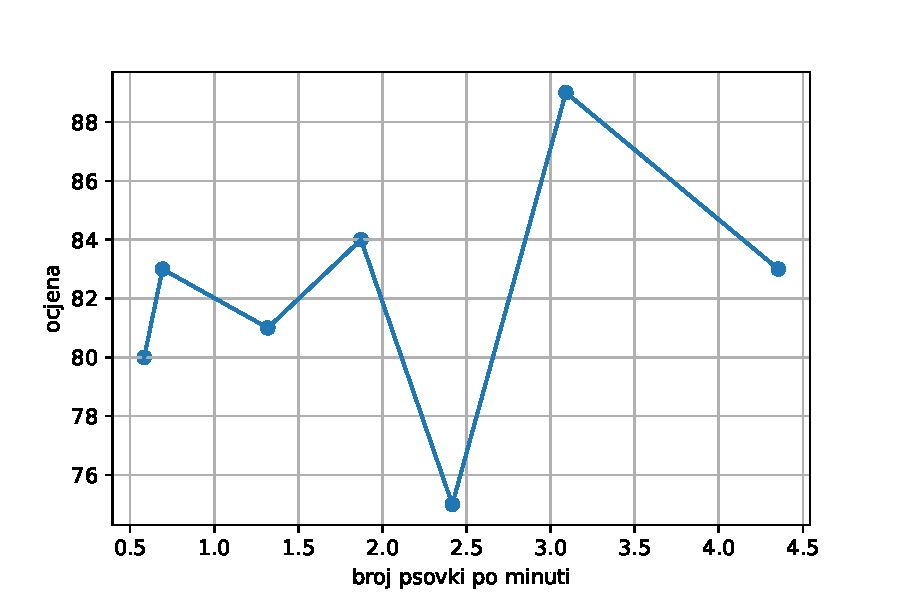
\includegraphics{"slike/psovke_po_minuti.pdf"}
	\caption{Usporedba ocjene s brojem psovki po minuti}
	\label{psovke_po_minuti}
\end{figure}

\paragraph{Distribucija vulgarnosti za vrijeme trajanja filma}

Idući zaključak kojeg bi bilo dobro donijeti je koja je distribucija
vulgarnosti za vrijeme trajanja filma. Ovi izvještaji su napravljeni tako da je
film vremenski podijeljen na trideset jednakih dijelova (neovisno o tome koliko
traje, dakle dužem filmu će jedna tridesetima duže trajati nego kratkom) te su
u tom razdoblju prebrojane psovke.

Za ovu svrhu se definira funkcija koja će davati graf s obzirom na to koje
argumente damo. Funkcija se definira ovako:
    \begin{tcolorbox}[breakable, size=fbox, boxrule=1pt, pad at break*=1mm,colback=cellbackground, colframe=cellborder]
\prompt{In}{incolor}{36}{\boxspacing}
\begin{Verbatim}[commandchars=\\\{\}]
\PY{k}{def} \PY{n+nf}{psovka\PYZus{}dio\PYZus{}filma}\PY{p}{(}\PY{n}{db\PYZus{}cursor}\PY{p}{,} \PY{n}{ime\PYZus{}filma}\PY{p}{,} \PY{n}{detail} \PY{o}{=} \PY{l+m+mi}{10}\PY{p}{,} \PY{n}{vulg} \PY{o}{=} \PY{l+s+s1}{\PYZsq{}}\PY{l+s+s1}{word}\PY{l+s+s1}{\PYZsq{}}\PY{p}{)}\PY{p}{:}
    \PY{n}{vulg} \PY{o}{=} \PY{l+s+s1}{\PYZsq{}}\PY{l+s+s1}{!}\PY{l+s+s1}{\PYZsq{}} \PY{k}{if} \PY{n}{vulg} \PY{o}{==} \PY{l+s+s1}{\PYZsq{}}\PY{l+s+s1}{word}\PY{l+s+s1}{\PYZsq{}} \PY{k}{else} \PY{l+s+s1}{\PYZsq{}}\PY{l+s+s1}{=}\PY{l+s+s1}{\PYZsq{}}
    \PY{n}{upit} \PY{o}{=} \PY{l+s+s1}{\PYZsq{}\PYZsq{}\PYZsq{}}
\PY{l+s+s1}{    SELECT CAST (rijec.vrijeme/film.trajanje*}\PY{l+s+si}{\PYZob{}0\PYZcb{}}\PY{l+s+s1}{ as INTEGER) as psovka\PYZus{}pc}
\PY{l+s+s1}{    FROM film, rijec}
\PY{l+s+s1}{    WHERE rijec.film\PYZus{}fk = film\PYZus{}id}
\PY{l+s+s1}{        AND rijec.rijec }\PY{l+s+si}{\PYZob{}2\PYZcb{}}\PY{l+s+s1}{= }\PY{l+s+s1}{\PYZsq{}}\PY{l+s+s1}{\PYZsq{}}
\PY{l+s+s1}{        AND film.naziv = }\PY{l+s+s1}{\PYZsq{}}\PY{l+s+si}{\PYZob{}1\PYZcb{}}\PY{l+s+s1}{\PYZsq{}}
\PY{l+s+s1}{    }\PY{l+s+s1}{\PYZsq{}\PYZsq{}\PYZsq{}}\PY{o}{.}\PY{n}{format}\PY{p}{(}\PY{n}{detail}\PY{p}{,} \PY{n}{ime\PYZus{}filma}\PY{p}{,} \PY{n}{vulg}\PY{p}{)}
    \PY{n}{data} \PY{o}{=} \PY{n}{db\PYZus{}cursor}\PY{o}{.}\PY{n}{execute}\PY{p}{(}\PY{n}{upit}\PY{p}{)}\PY{o}{.}\PY{n}{fetchall}\PY{p}{(}\PY{p}{)}
    \PY{n}{fig}\PY{o}{.}\PY{n}{tight\PYZus{}layout}\PY{p}{(}\PY{p}{)}
    \PY{n}{ax}\PY{o}{.}\PY{n}{grid}\PY{p}{(}\PY{k+kc}{True}\PY{p}{)}
    \PY{n}{ax}\PY{o}{.}\PY{n}{bar}\PY{p}{(}\PY{n}{data}\PY{o}{.}\PY{n}{keys}\PY{p}{(}\PY{p}{)}\PY{p}{,} \PY{n}{data}\PY{o}{.}\PY{n}{values}\PY{p}{(}\PY{p}{)}\PY{p}{)}
    \PY{n}{plt}\PY{o}{.}\PY{n}{savefig}\PY{p}{(}\PY{l+s+s2}{\PYZdq{}}\PY{l+s+s2}{rad/slike/}\PY{l+s+s2}{\PYZdq{}} \PY{o}{+} \PY{n}{ime\PYZus{}filma} \PY{o}{+} \PY{l+s+s2}{\PYZdq{}}\PY{l+s+s2}{\PYZus{}}\PY{l+s+s2}{\PYZdq{}} \PY{o}{+} \PY{n}{vulg} \PY{o}{+} \PY{l+s+s2}{\PYZdq{}}\PY{l+s+s2}{.pdf}\PY{l+s+s2}{\PYZdq{}}\PY{p}{)}
\end{Verbatim}
\end{tcolorbox}

Jedan poziv ove funkcije izgleda:

\begin{tcolorbox}[breakable, size=fbox, boxrule=1pt, pad at break*=1mm,colback=cellbackground, colframe=cellborder]
\prompt{In}{incolor}{37}{\boxspacing}
\begin{Verbatim}[commandchars=\\\{\}]
\PY{n}{psovka\PYZus{}dio\PYZus{}filma}\PY{p}{(}\PY{n}{c}\PY{p}{,} \PY{l+s+s1}{\PYZsq{}}\PY{l+s+s1}{Kill Bill: Vol. 2}\PY{l+s+s1}{\PYZsq{}}\PY{p}{,} \PY{n}{detail} \PY{o}{=} \PY{l+m+mi}{20}\PY{p}{,} \PY{n}{vulg}\PY{o}{=}\PY{l+s+s1}{\PYZsq{}}\PY{l+s+s1}{word}\PY{l+s+s1}{\PYZsq{}}\PY{p}{)}
\end{Verbatim}
\end{tcolorbox}

\begin{figure}
	\centering
	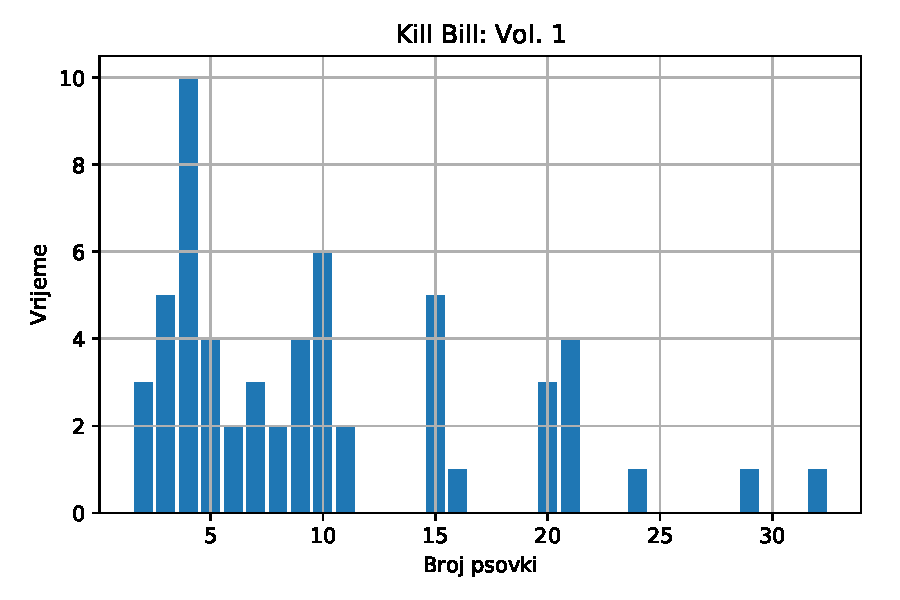
\includegraphics{"slike/Kill Bill: Vol. 1_!.pdf"}
	\caption{Prikaz distribucije psovki u filmu \textit{Kill Bill: Vol. 1}}
	\label{distribucija_psovki}
\end{figure}

A istu funkciju možemo pustiti i kroz petlju i dobiti sliku za svaki film u
stupčastom dijagramu (slika \ref{distribucija}).

\begin{figure*}[h]
    \centering
    \begin{subfigure}[t]{0.5\textwidth}
        \centering
        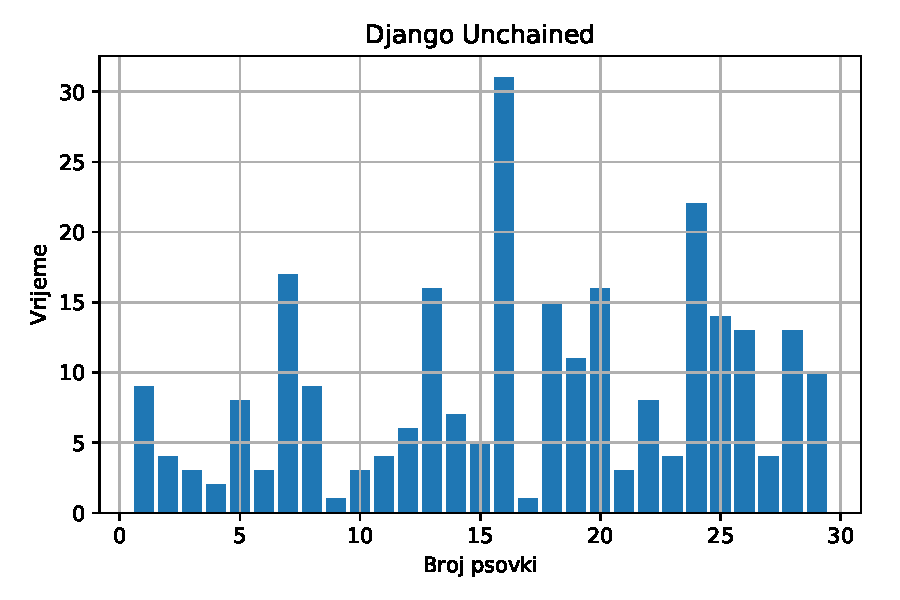
\includegraphics{slike/django.pdf}
    \end{subfigure}%
    \begin{subfigure}[t]{0.5\textwidth}
        \centering
        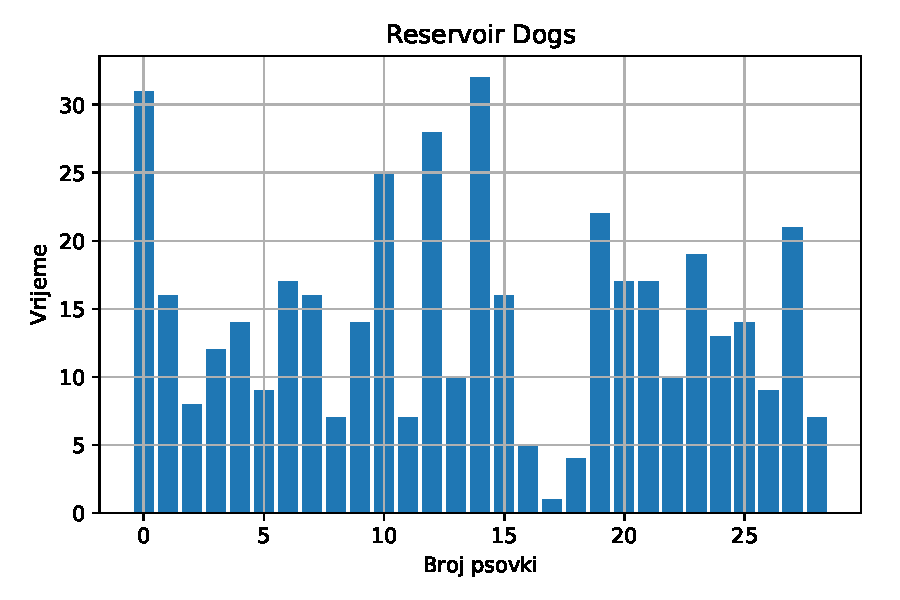
\includegraphics{slike/dogs.pdf}
    \end{subfigure}\\
    \begin{subfigure}[t]{0.5\textwidth}
        \centering
        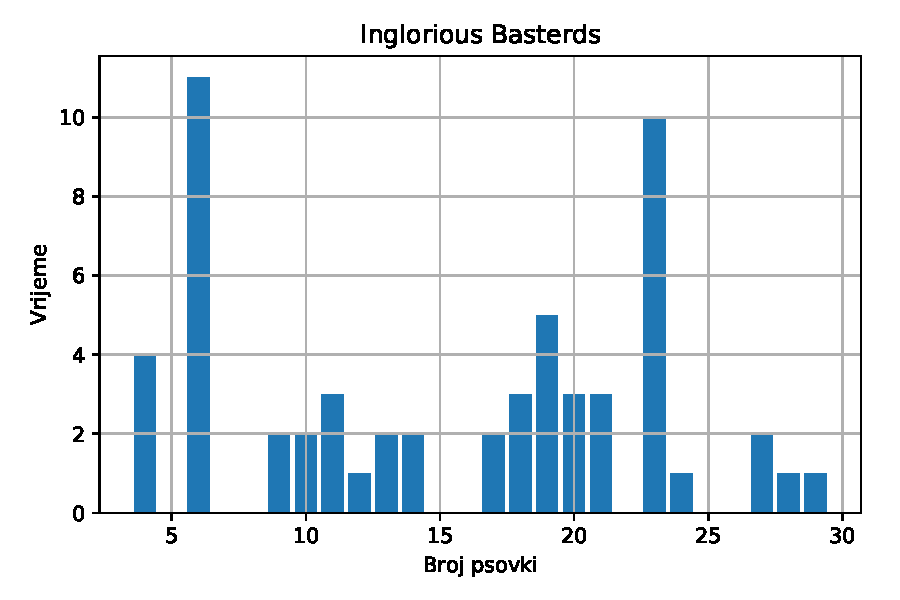
\includegraphics{slike/bastards.pdf}
    \end{subfigure}%
    \begin{subfigure}[t]{0.5\textwidth}
        \centering
        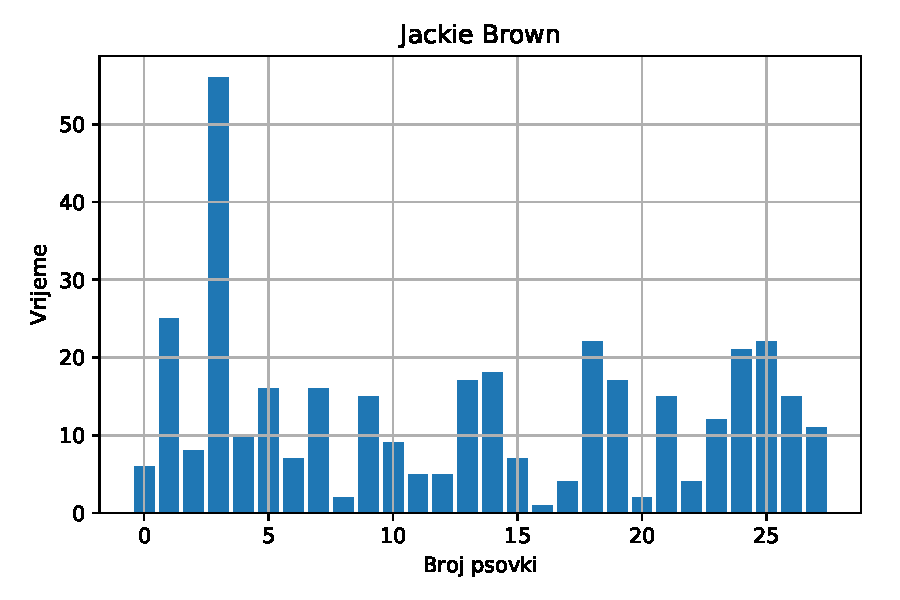
\includegraphics{slike/jackie.pdf}
    \end{subfigure}\\
    \begin{subfigure}[t]{0.5\textwidth}
        \centering
        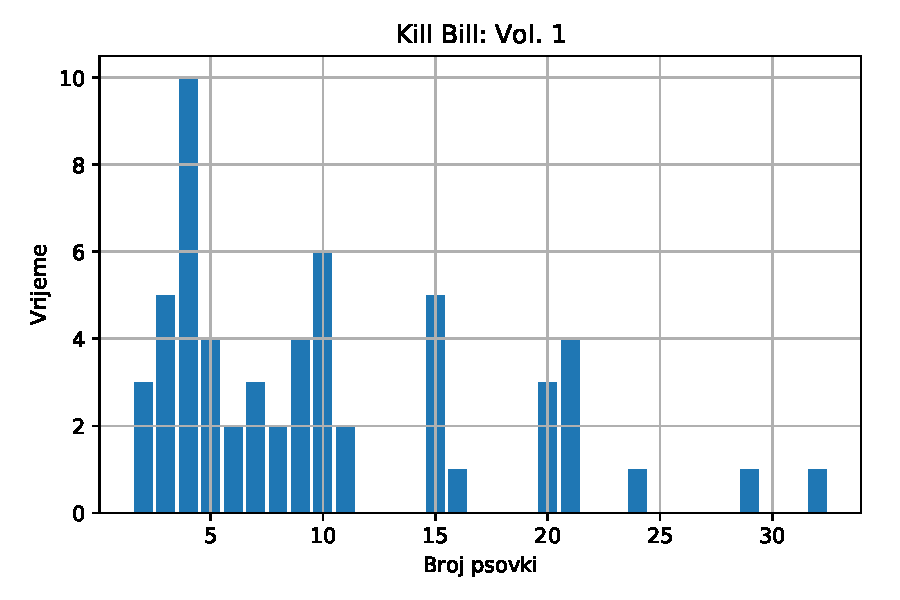
\includegraphics{slike/kill1.pdf}
    \end{subfigure}%
    \begin{subfigure}[t]{0.5\textwidth}
        \centering
        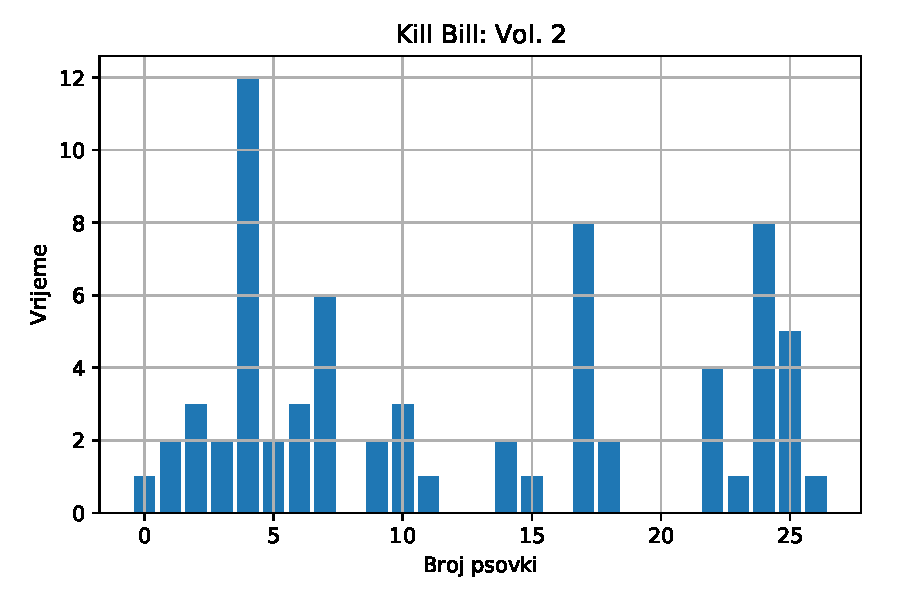
\includegraphics{slike/kill2.pdf}
    \end{subfigure}\\
    \begin{subfigure}[t]{0.5\textwidth}
        \centering
        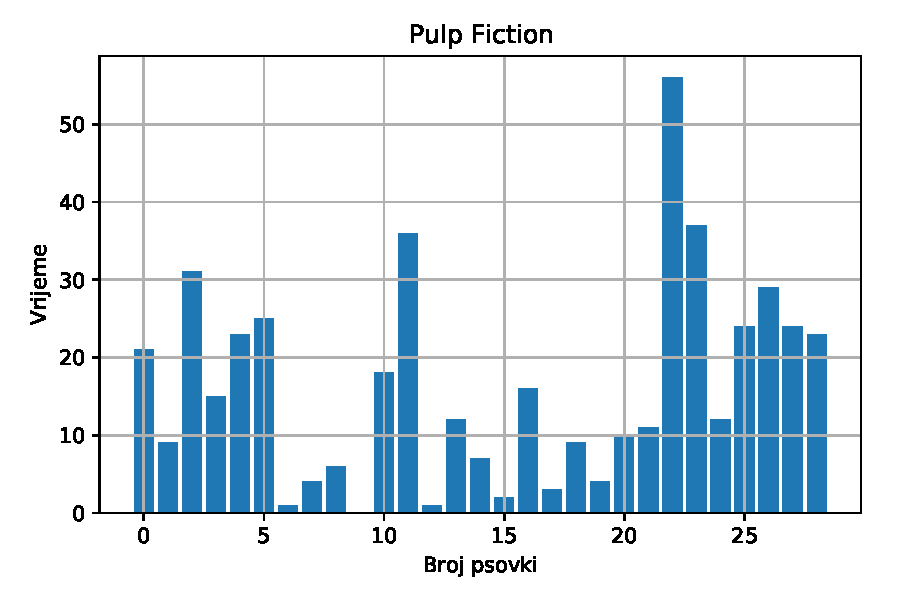
\includegraphics{slike/pf.pdf}
    \end{subfigure}\\
    \caption{Prikaz distribucije psovki po filmovima}
	\label{distribucija}
\end{figure*}

Iz dijagrama (slika \ref{distribucija_psovki}) može se vidjeti koji filmovi
imaju veću koncentraciju u kojem dijelu, odnosno kako su psovke distribuirane
kroz film.

\begin{figure}[h]
	\centering
	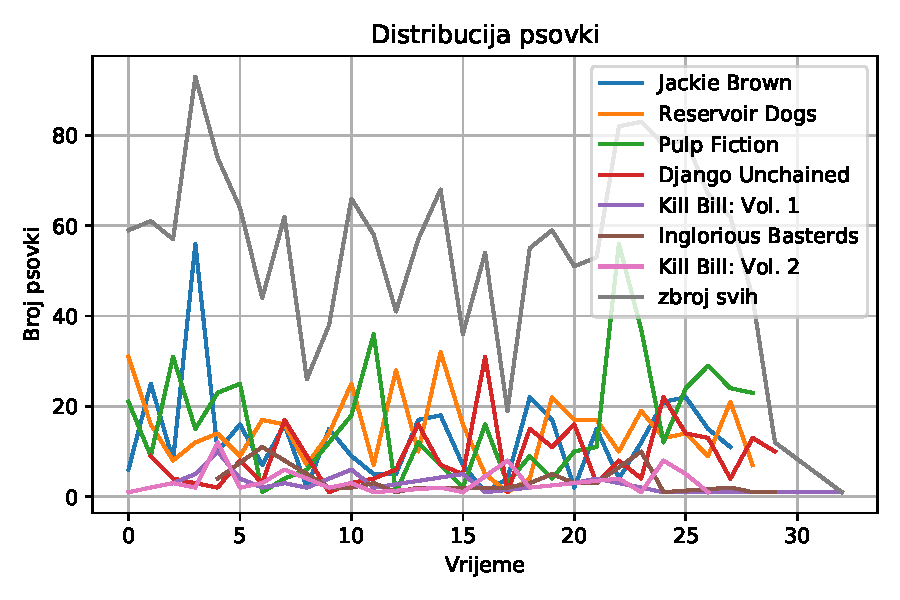
\includegraphics{"slike/filmovi_distribucija_psovki.pdf"}
	\caption{Prikaz distribucije psovki u svim filmovima}
	\label{distribucija_psovki}
\end{figure}

\paragraph{Količina psovki kroz godine}

Iduće što je korisno za analizirati je kako se broj psovki kretao kroz godine
(slika \ref{psovke_godine}.  Za ovaj primjer također će se gledati prosjek po
minuti, a ne apsolutan broj.

\begin{figure}[h]
	\centering
	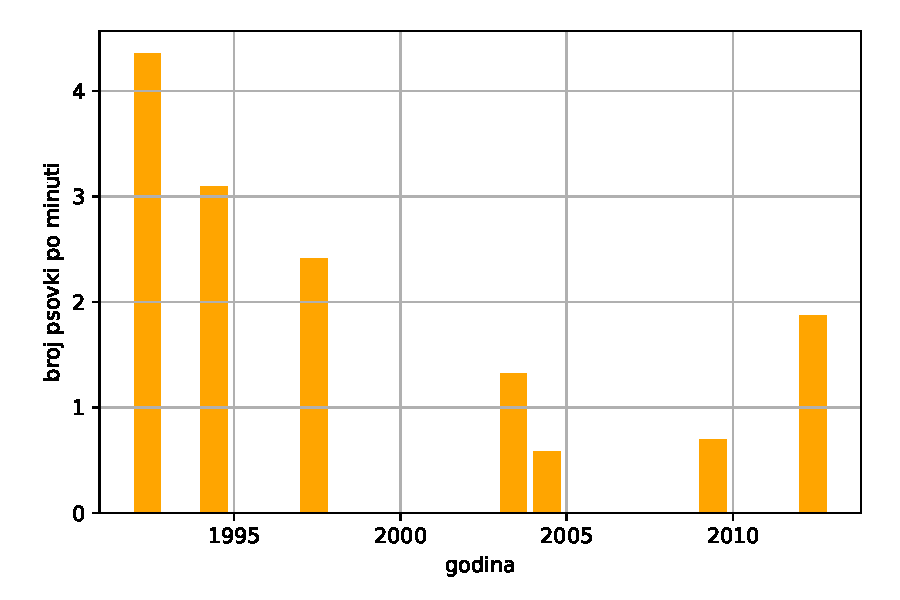
\includegraphics{"slike/psovke_godine.pdf"}
	\caption{Trendovi psovki po godinama}
	\label{psovke_godine}
\end{figure}

\paragraph{Kategorizacija psovki}

Iz odabranih filmova može se i pogledati koje su se kategorije psovki najčešće
izgovarale. Psovke su kategorizirane prema temi na koju se odnose. Ovisno o
tome koliko je ova podjela dobro napravljena, toliko će se lako moći isčitati
rezultati o zastupljenosti pojedinih psovki stoga je dobra ideja detaljno
proučiti značenje svakih od izraza kako bi se dobilo što jasnije rješenje.

\begin{figure}[h]
	\centering
	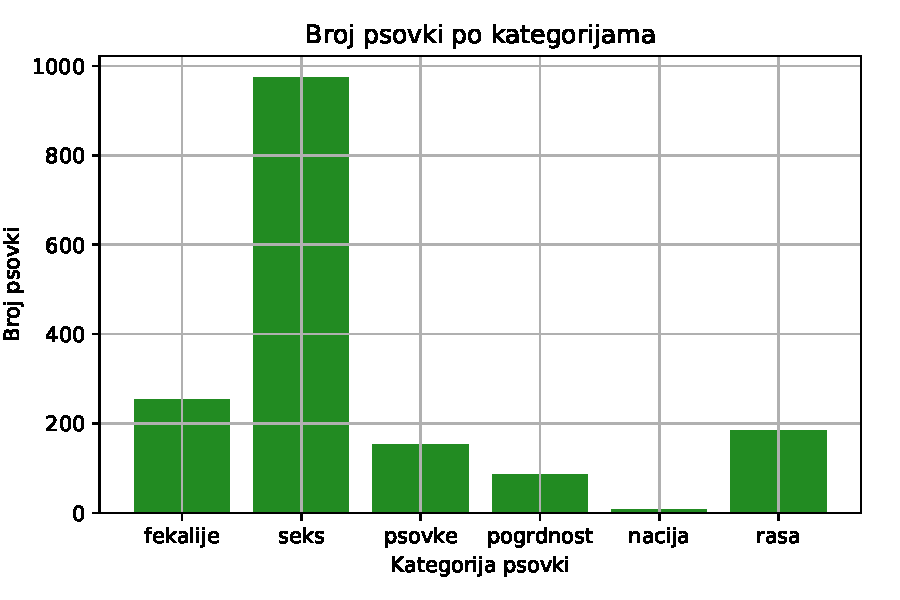
\includegraphics{"slike/kategorije_total.pdf"}
	\caption{Broj psovki po kategorijama}
	\label{psovke_po_kat}
\end{figure}

Ono što je također značajno za vidjeti je kako su koje psovke zastupljene po
filmovima. Prema grafu na slici \ref{psovke_po_kat_po_film} vidi se da su u
Pulp Fictionu najzastupljenije psovke vezane za seksualne teme, a rasistički
se izrazi najviše koriste u Django Unchainedu.

\begin{figure}[h]
	\centering
	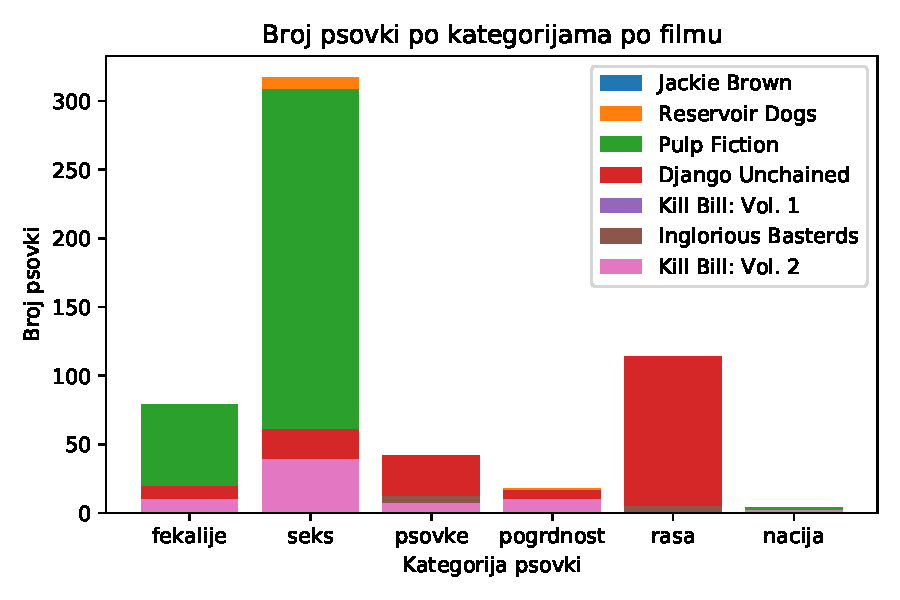
\includegraphics{"slike/kategorije_total_po_filmovima.pdf"}
	\caption{Broj psovki po kategorijama}
	\label{psovke_po_kat_po_film}
\end{figure}

\chapter{Zaključak}

Kroz ovaj projekt pokazale su se osnovne značajke skladišta podataka. Zbog vrlo
malenog \textit{dataseta} nije moguće u potpunosti demonstrirati sve
funkcionalnost i prednosti skladišta nad bazama u svrhu izvještavanja, no
vodeći se ovim primjerima nastala skladišta u puno većim razmjerima bi
zasigurno pokazala bolje performanse i lakoću izrade izvještaja.

Ovaj projekt je također i pokazao kako se na vrlo jednostavan način mogu
spojiti tehnologije koje djeluju na puno nižoj razini apstrakcije od, npr.
\textit{SQL Management Studija}, a bez mnogo kompliciranja u obradi podataka.
To nam je omogućio Python kojemu je specijalnost jednostavno rukovanje
podatcima na jednostavan, a opet učinkovit način.

Također, \texttt{SQLite} je jedinstven sustav za upravljanje bazom jer nema
potrebu za serverom, odnosno sve je spremljeno u jednoj datoteci i tako se
dobro nadovezuje na skup tehnologija koje su se koristile do tada. Jupyter
Notebook također je odličan za ovaku primjenu jer omogućuje jednostavnu
vizualizaciju svega što se crta te ima jednostavan pregled koda.

Sve u svemu, tehnologije koje su demonstrirane dobro služe ovoj svrsi i kad se
koriste na kvalitetan način čine ekosustav za upravljanje podatcima na
elegantan i efikasan način. Skladište je usredotočeno na brojenje riječi po
određenim kriterijima te izvještaji omogućuju mjerenje količine i distribucije
psovki po filmovima na puno načina.

\begin{appendices}
\chapter{Jupyter Notebook bilježnica s cijelim procesom}
\centering
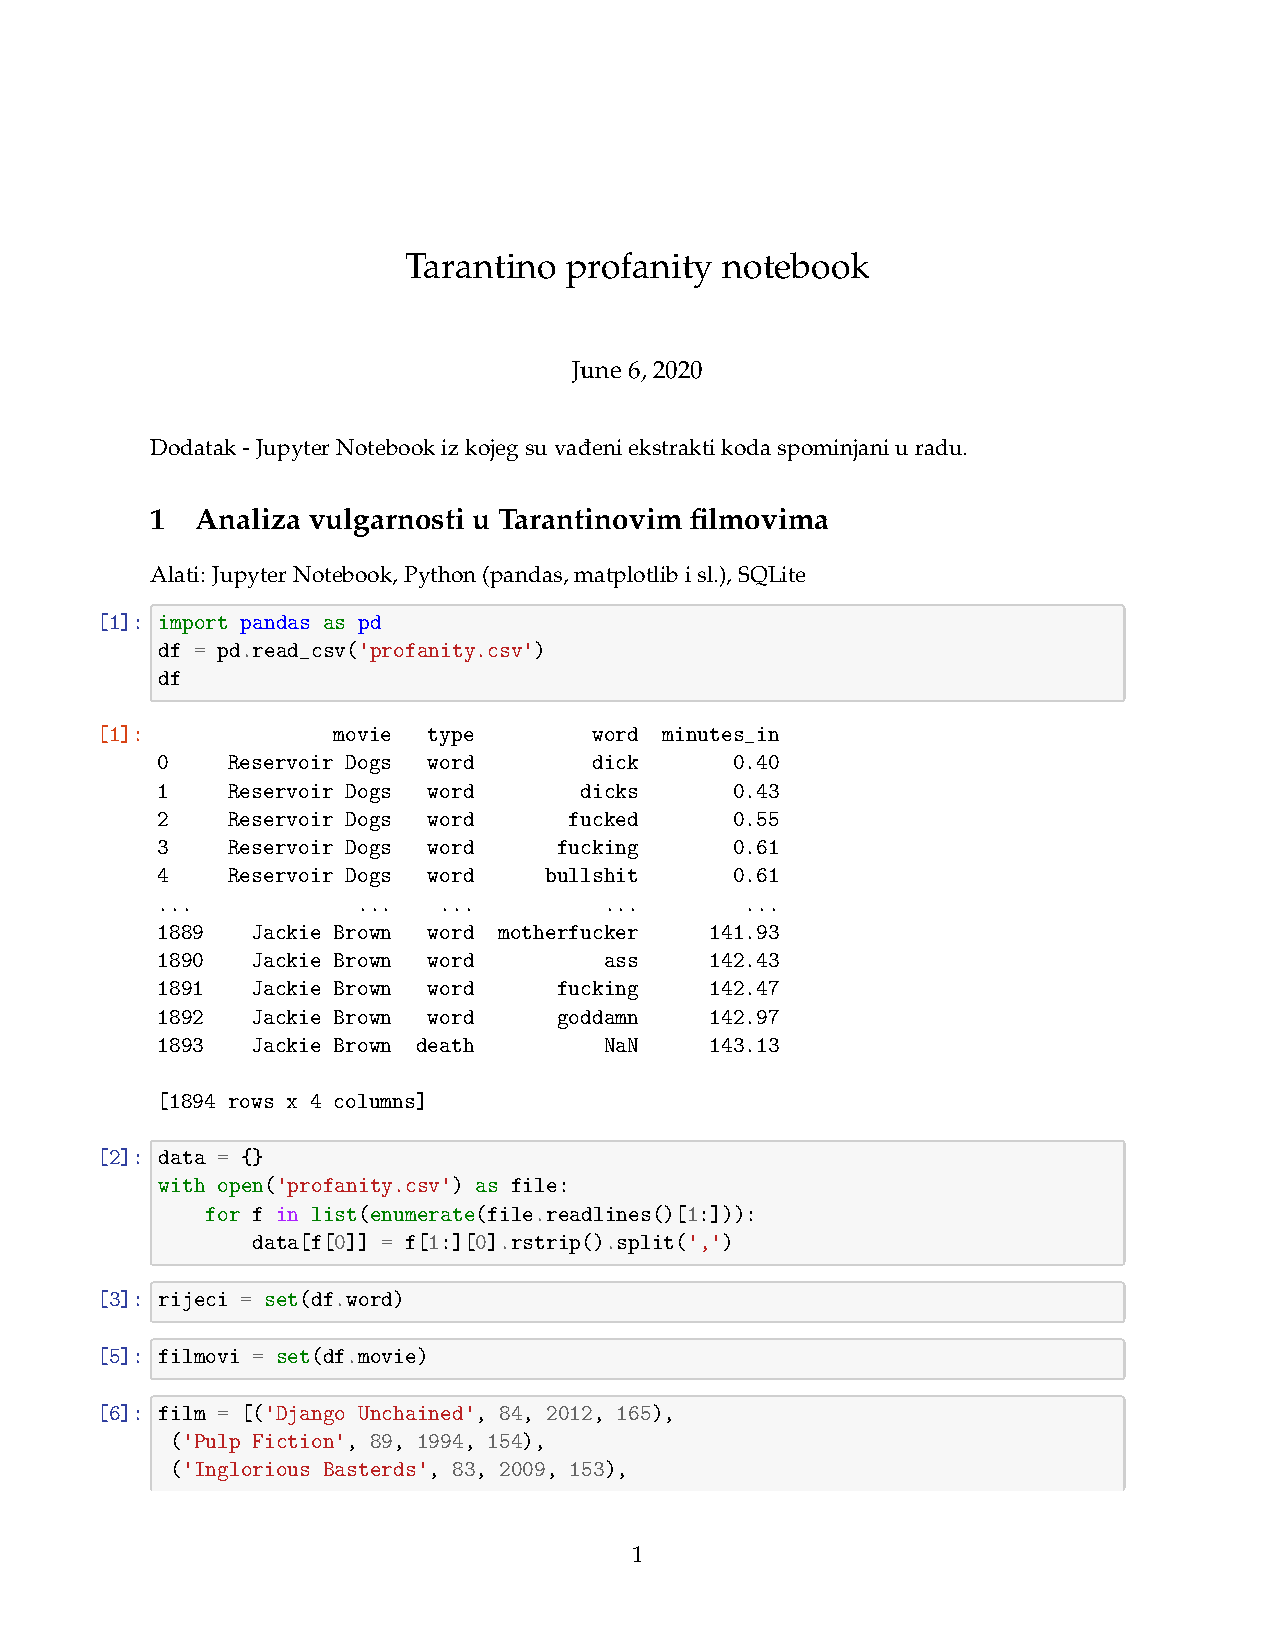
\includegraphics[page=1, scale=1.2]{notebook/nb.pdf}
\includepdf[pages=2-]{notebook/nb.pdf}
\end{appendices}

\end{document}
